\documentclass{article}
\usepackage[greek,english]{babel}
\usepackage[utf8x]{inputenc}
\usepackage{natbib}
\usepackage{graphicx}
\usepackage{subfigure}
\graphicspath{ {.//} }
\usepackage{xcolor}
\graphicspath{ {./images/} }
\usepackage{titling}
\setlength{\droptitle}{10em}
\title{%
  \selectlanguage{greek}\Huge
 Μοντέλα υπολογιστικού νέφους \\}
\begin{document}
\selectlanguage{greek}
\author{\selectlanguage{greek}\LARGE
  Γεώργιος Νικολάου\\
   \texttt{\selectlanguage{english}\large sdi1800134}
  \and
  \selectlanguage{greek}\LARGE
  Νεφέλη Ταβουλάρη\\
   \texttt{\selectlanguage{english}\large sdi1800190}
}
\maketitle


\begin{figure}
\centering
\begin{subfigure}
  \centering
  
\includegraphics[width=40mm]{dit_logo}
  \label{fig:sub1}
\end{subfigure}%
\begin{subfigure}
  \centering
  
\includegraphics[width=50mm]{NKUA_logo}
  \label{fig:sub2}
\end{subfigure}
\label{fig:test}
\end{figure}


\newpage
\tableofcontents
\newpage
\section{Περίληψη}
Σε αυτή τη μελέτη θα προσπαθήσουμε να αναλύσουμε τις νέες τάσεις στην ανάπτυξη Πληροφοριακών Συστημάτων, δίνοντας έμφαση στο Υπολογιστικό Νέφος και μερικά από τα πιο γνωστά μοντέλα του. Με αυτό τον τρόπο θα κατανοήσουμε τα πλεονεκτήματα και τα μειονεκτήματα αυτών των λύσεων ,θα εμβαθύνουμε παραθέτοντας παραδείγματα και θα βγάλουμε συμπεράσματα κάνοντας συγκρίσεις μεταξύ τους.
\section{Εισαγωγή}
\subsection{Η Ανάγκη για Πληροφοριακά Συστήματα}
Διανύουμε την τέταρτη τεχνολογική επανάσταση και αρκεί μια ματιά γύρω μας για να καταλάβουμε πως ζούμε σε μια εποχή ταχύτατων αλλαγών. Χάρη στην ανάπτυξη και την εύκολη πρόσβαση σε νέα τεχνολογικά προϊόντα, οι άνθρωποι έχουν ταυτόχρονα τη δυνατότητα αλλά και την ανάγκη να επικοινωνούν και να αλληλεπιδρούν, ο ένας με τον άλλο αλλά και με τις επιχειρήσεις, τους δημόσιους οργανισμούς ή/και τους άλλους φορείς που συνθέτουν τον σύγχρονο κόσμο που τους περιβάλλει, με ταχύτητα, αμεσότητα και συχνά μεταδίδοντας μεγάλο όγκο σύνθετων δεδομένων. Ακόμα, οι σχέσεις μεταξύ των παραπάνω γίνονται προοδευτικά όλο και πιο πολύπλοκες, σύνθετες και μεταβαλλόμενες με όλο και αυξανόμενη ταχύτητα για να προσαρμοστούν στην εξ’ ίσου γρήγορα μεταβαλλόμενη πραγματικότητα της σύγχρονης κοινωνικοοικονομικής ζωής. Για την παραγωγή και την διάθεση στην αγορά των σύγχρονων, προϊόντων και υπηρεσιών απαιτούνται συνήθως σύνθετες εφοδιαστικές αλυσίδες, τα επιμέρους στοιχεία των οποίων, όπως επίπεδα διαθέσιμου προϊόντος σε μια αποθήκη ή η θέση ενός φορτηγού εφοδιασμού συλλέγονται, αποθηκεύονται και επεξεργάζονται μέσα από ένα δαιδαλώδες δίκτυο αισθητήρων που συλλέγουν τα δεδομένα  και υπολογιστών ή/και διακομιστών που πρέπει να τα αποθηκεύσουν και να τα επεξεργαστούν, συνθέτοντας έτσι αυτό που ονομάζουμε διαδίκτυο των πραγμάτων \selectlanguage{english}(Internet of Things). \selectlanguage{greek}Η αποτελεσματική επεξεργασία και αποθήκευση των πληροφοριών που προκύπτουν από αυτή τη διαδικασία αποτελεί στόχο κάθε οργανισμού που στοχεύει στην μείωση των λειτουργικών του εξόδων και αύξηση των εσόδων, είναι επομένως υψίστης σημασίας, γίνεται δε όλο και πιο περίπλοκη καθώς οι ρυθμοί της σύγχρονης αγοράς επιταχύνουν. Ακόμα, η μεγάλη πρόοδος της επιστήμης της πληροφορικής στον κλάδο της Τεχνητής Νοημοσύνης (\selectlanguage{english}A.I.) \selectlanguage{greek}και συγκεκριμένα της Μηχανικής Μάθησης (\selectlanguage{english}Machine Learning) \selectlanguage{greek}έχει επιτρέψει την δημιουργία έξυπνων μοντέλων που είναι σε θέση να προβλέψουν με μεγάλη ακρίβεια φυσικά, οικονομικά ή άλλα φαινόμενα που επιτρέπουν στις εταιρίες να αναπτύξουν και να διανείμουν τα προϊόντα και τις υπηρεσίες τους και να σχεδιάσουν την επιχειρηματική τους δράση σε όλα τα επίπεδα όπως ποτέ πριν. Για να μπορέσουν όμως να δημιουργηθούν τα μοντέλα αυτά πρέπει να “εκπαιδευτούν” πάνω στα δεδομένα που περιγράφουν το πρόβλημα, τα οποία στο σύγχρονο περιβάλλον είναι πολλά και πολύπλοκα, και αυξάνουν με ραγδαίους ρυθμούς. Είναι φανερό, λοιπόν, πως για να μπορέσουν οι φορείς οι οποίοι δραστηριοποιούνται στο περιβάλλον αυτό να ρυθμίσουν την λειτουργία τους, να σχεδιάσουν το μέλλον τους, να θέσουν στόχους και να τους πετύχουν, πρέπει να  είναι σε θέση να κατανοήσουν ένα εξαιρετικά ογκώδες και σύνθετο σύνολο δεδομένων, το οποίο αλλάζει σε δομή και περιεχόμενο με μεγάλη ταχύτητα.
Έπεται, έτσι, πως η σύγχρονη κοινωνία, και όσοι δραστηριοποιούνται σε αυτή, έχουν ανάγκη από εξελιγμένα πληροφοριακά συστήματα
Δεν αρκεί όμως απλά  να βρεθεί τρόπος να κατανοήσει κάνεις τα δεδομένα και να εξάγει συμπεράσματα από αυτά. Πρέπει αυτό να γίνει γρήγορα, με μεγάλη βεβαιότητα ως προς το αποτέλεσμα, με μέσα αξιόπιστα ως προς την λειτουργία τους και με το μικρότερο δυνατό κόστος.


\begin{itemize}
\item Γρήγορα, καθώς για να μπορέσει να είναι χρήσιμη στον προγραμματισμό του οργανισμού μια πληροφορία, πρέπει να μπορεί να φτάσει στα χέρια των στελεχών που θα λάβουν απόφαση σε ένα εύλογο χρονικό διάστημα. Αν φτάσει καθυστερημένα σε βαθμό που η απόφαση δεν προλαβαίνει να εφαρμοστεί, όχι απλά δεν υπάρχει κάποιο όφελος, αλλά έχουν χαθεί όλοι οι πώροι που δαπανήθηκαν για να φτάσουμε στην πληροφορία αυτή.
\item Βεβαιότητα για το αποτέλεσμα καθώς ακόμα και μικρά λάθη ή ατέλειες, λειτουργώντας συσσωρευτικά θα δημιουργήσουν αυξημένο κόστος για τον οργανισμό.
\item Αξιόπιστα, καθώς ακόμα και μικρή παύση της λειτουργίας ενός πληροφοριακού συστήματος ενδέχεται να έχει καταστροφικές συνέπειες και να οδηγήσει σε χαμένες ευκαιρίες με μεγάλο οικονομικό αντίκτυπο. Είναι εύκολο να φανταστούμε τις συνέπειες από την κατάρρευση ενός συστήματος λόγω πίεσης, παραδείγματος χάρη σε μια περίοδο αυξημένου όγκου παραγγελιών ενός προϊόντος.
\item Φθηνά, καθώς ο σκοπός ύπαρξης τέτοιων συστημάτων είναι η μείωση του κόστους λειτουργίας και η μεγιστοποίηση των κερδών. Αν το όφελος υπερκαλυφθεί από το κόστος πρόσκτησης και λειτουργίας του συστήματος, τότε αυτό αποτελεί δώρον άδωρον.
\end{itemize}

\subsection{Τα Σύγχρονα Πληροφοριακά Συστήματα}
Για να βρεθεί λύση στα ζητήματα αυτά, ο κλάδος της πληροφορικής έχει στραφεί σε νέες  μεθόδους διαχείρισης της πληροφορίας και σχεδίασης λογισμικού. Ας εξετάσουμε μερικά παραδείγματα:

\begin{itemize}
\item Ο κλάδος της Ανάλυσης Μαζικών Δεδομένων \selectlanguage{english}(Big Data Computing), \selectlanguage{greek}πραγματεύεται την αναζήτηση μεθόδων αποτελεσματικού χειρισμού μεγάλου όγκου δεδομένων,συμπεριλαμβανομένων ζητημάτων ως προς την αποτελεσματική αποθήκευση, ανάλυση και ασφάλεια των δεδομένων μεταξύ άλλων ζητημάτων. Χαρακτηρίζεται από τις τρεις λέξεις κλειδιά “Όγκος, Ταχύτητα, Ποικιλομορφία”, γνωστές και ως τα “3 \selectlanguage{english}Vs” (volume, variety, velocity) \selectlanguage{greek}που περιγράφουν την μεγάλη ταχύτητα εισροής και μεταβολής των δεδομένων, τους πολλούς διαφορετικούς τύπους δεδομένων που περιγράφουν ένα αντικείμενο ή φαινόμενο, και φυσικά τον μεγάλο όγκο. Συχνά εφαρμόζονται σε προβλήματα χρηματιστηριακών προβλέψεων \selectlanguage{english}(FinTech), \selectlanguage{greek}προβλήματα Ανάλυσης Συμπεριφοράς Χρηστών \selectlanguage{english}(User Behaviour Analysis) \selectlanguage{greek}και προβλήματα πρόβλεψης φυσικών/ιατρικών φαινομένων, όπως ακραία καιρικά φαινόμενα και επιδημίες αντίστοιχα.
\item Η ευέλικτη μεθοδολογία \selectlanguage{english}(Agile development) \selectlanguage{greek}αποτελεί ένα σύνολο αρχών βάσει των οποίων αυτοοργανωτικές και διαλειτουργικές ομάδες αναπτύσσουν λογισμικό χρησιμοποιώντας προσαρμοστικό σχεδιασμό, εξελικτική ανάπτυξη και έγκαιρη παράδοση / συνεχή βελτίωση, με στόχο την μείωση του χρόνου ανάπτυξης και κατά συνέπεια του κόστους ώστε να αμβλυνθούν τα προβλήματα που προκύπτουν απο την μεταβολή της κατανόησης του προβλήματος και τον επαναπροσδιορισμό των στόχων που προκύπτουν κατά τη σχεδιαστική διαδικασία.
\item Το \selectlanguage{english}DevOps, \selectlanguage{greek}όπως ονομάζεται, αποτελεί ένα σύνολο φιλοσοφιών, μεθόδων και εργαλείων που, ομοίως με την ευέλικτη μεθοδολογία, έχουν ως στόχο την επιτάχυνση της ανάπτυξης λογισμικού μέσα από αυξημένη προσαρμοστικότητα στις αλλαγές που προκύπτουν κατά την σχεδίαση και υλοποίηση. Διαφοροποιείται από την παραπάνω μέθοδο σε δύο κυρίως τομείς, στην έμφαση που δίνει στον κύκλο ανατροφοδότησης μεταξύ ομάδες σχεδιασμού και πελάτη με στόχο την συνεχή βελτίωση του προϊόντος, αλλά και στην στενή συνεργασία των ομάδων σχεδίασης / υλοποίησης και των ομάδων που θα λειτουργήσουν το τελικό προϊόν, ώστε να επιτευχθεί λύση που είναι κοντά στις απαιτήσεις των δεύτερων.
\item Η \selectlanguage{english}microservice\selectlanguage{greek} αρχιτεκτονική είναι η νέα τάση στην ανάπτυξη λογισμικού. Η δημιουργία μονολίθων, δηλαδή ενός ενιαίου συστήματος, αρχίζει να καταργείται. Η κάθε "μικροϋπηρεσία" είναι αυτόνομη, με αποτέλεσμα να είναι εύκολη η πρόσθεση, αφαίρεση, ανανέωση κάποιων από αυτές, χωρίς να χρειάζεται να μεταβληθούν οι υπόλοιπες, ενώ είναι δυνατό συγκεκριμένες υπηρεσίες να υλοποιηθούν με χρήση εμπορικού λογισμικού “από το ράφι” (\selectlanguage{english}off the shelf software) \selectlanguage{greek}εξοικονομώντας χρόνο και χρήμα.
Έτσι, επιτυγχάνεται ευελιξία, κλιμάκωση, καινοτομία, ταχύτητα. Οι\selectlanguage{english} developers \selectlanguage{greek}μπορούν πιο εύκολα να παίρνουν πρωτοβουλίες και αποφάσεις , καθώς δεν εξαρτάται από αυτούς ολόκληρη η εφαρμογή. Με αυτό τον τρόπο, είναι και ευκολότερη η διαχείριση προβλημάτων, καθώς αυτά απομονώνονται. Αυξάνεται, λοιπόν, η απόδοση, η ποιότητα του λογισμικού, η συνεργασία, η ασφάλεια των δεδομένων, η διατηρησιμότητα. 
Σε συνδυασμό με τη χρήση \selectlanguage{english}REST API's,\selectlanguage{greek} μια εταιρεία μπορεί για παράδειγμα να αλλάξει το \selectlanguage{english}frontend \selectlanguage{greek}μιας εφαρμογής, με σκοπό να χρησιμοποιήσει μια πιο σύγχρονη γλώσσα, με μεγάλη ευκολία και ταχύτητα.
\item Μια προσέγγιση που αποσκοπεί στην διευκόλυνση της διαχείρισης μεγάλων όγκων δεδομένων ακούει στο όνομα \selectlanguage{english}Edge Computing\selectlanguage{greek}, το οποίο αποτελεί ένα υπολογιστικό “σχήμα" βάσει του οποίου η επεξεργασία και αποθήκευση των δεδομένων λαμβάνει χώρα κοντά στην πηγή τους, ιδανικά και από την ίδια συσκευή που παράγει τα δεδομένα, με σκοπό τη μείωση του χρόνου απόκρισης και της κατανάλωσης πόρων του δικτύου καθώς τα δεδομένα διανύουν μικρότερη απόσταση μέσα σε αυτό. Συγγενικό είναι και το σχήμα \selectlanguage{english}Fog Computing\selectlanguage{greek}, που διαφοροποιείται από το \selectlanguage{english}Edge Computing\selectlanguage{greek} στην τοπολογία, με την επεξεργασία και αποθήκευση να λαμβάνει χώρο σε μια ή περισσότερες συσκευές συνδεδεμένες στις πηγές των δεδομένων σε ένα τοπικό δίκτυο.


\end{itemize}
Η πιο αποφασιστική απάντηση στα προβλήματα αυτά όμως, η οποία επιτρέπει και την εφαρμογή των αρχών που συζητήσαμε παραπάνω, δίνεται από το υπολογιστικό νέφος \selectlanguage{english}(Cloud Computing), \selectlanguage{greek}μια επαναστατική τεχνολογία που θα αναλύσουμε με λεπτομέρεια παρακάτω.




\section{Υπολογιστικό Νέφος}
Αρχικά, θεωρούμε αναγκαίο να κάνουμε μια σύντομη ανάλυση των κύριων χαρακτηριστικών του Υπολογιστικού Νέφους, ώστε να είμαστε σε θέση να κατανοήσουμε και τη σημασία ολόκληρης της μελέτης μας , αλλά και με σκοπό να σκεφτούμε συνδυαστικά τις διάφορες σύγχρονες έννοιες.
\subsection{Ορισμός}
Με βάση τον ορισμό του\selectlanguage{english} NIST \selectlanguage{greek}(Εθνικό Ίδρυμα για τα Πρότυπα και την Τεχνολογία), το Υπολογιστικό Νέφος έιναι ένα μοντέλο που επιτρέπει μια πανταχού παρούσα και με βάση τη ζήτηση \selectlanguage{english}(on demand, pay-per-use)\selectlanguage{greek} δικτυακή σύνδεση σε διαμοιρασμένους υπολογιστικούς πόρους (πχ δίκτυο, αποθήκευση, εφαρμογές, υπηρεσίες, σέρβερς), που μπορούν γρήγορα και εύκολα να υπολογιστούν και να διατεθούν από έναν πάροχο.
\subsection{Οφέλη}
Ένα από τα σημαντικότερα πλεονεκτήματα του Υπολογιστικού Νέφους, που φυσικά ενδιαφέρει πολύ τις επιχειρήσεις είναι η μείωση του κόστους, η οποία οφείλεται σε πολλά και διαφορετικά χαρακτηριστικά του Νέφους. Τα οποία είναι τα εξής:
\begin{itemize}
\item	Μετακινώντας τις εφαρμογές του στο Νέφος, o καταναλωτής Νέφους \selectlanguage{english}(Cloud Consumer)\selectlanguage{greek} απαλλάσσεται από τα έξοδα για την απόκτηση και τη συντήρηση εξοπλισμού \selectlanguage{english}(capital expenditure),\selectlanguage{greek} καθώς ο απαιτούμενος εξοπλισμός ή μέρος αυτού δε βρίσκεται στις εγκαταστάσεις της εταιρείας \selectlanguage{english}(on premises) \selectlanguage{greek},αλλά σε \selectlanguage{english}Data Centers.\selectlanguage{greek}

\item	Ο καταναλωτής πληρώνει για όσα χρησιμοποιεί\selectlanguage{english} ( pay-as-you-go )\selectlanguage{greek} , δεν υποαπασχολεί πόρους , ούτε χρησιμοποιεί πόρους που δε χρειάζεται . Γι’ αυτό και παλιότερα το\selectlanguage{english} Cloud Computing \selectlanguage{greek}ονομαζόταν\selectlanguage{english} Utility Computing. \selectlanguage{greek}Αυτό συμβαίνει διότι, με διάφορες στρατηγικές \selectlanguage{english}(lag strategy, lead strategy, match strategy),\selectlanguage{greek} ο χρήστης έχει τη δυνατότητα να αυξομειώνει τις εικονικές μηχανές ή όποιον άλλο πόρο, είτε προληπτικά, είτε ύστερα από την υπέρβαση κάποιου ορίου\selectlanguage{english}/threshold,\selectlanguage{greek} αλλά και να ελαχιστοποιεί το κόστος του.

\item	Οι εταιρείες που μεταφέρονται στο Νέφος, έχουν την ευκαιρία να αφοσιωθούν στο έργο τους, καθώς εξοικονομείται όλος ο χρόνος και η προσπάθεια που απαιτεί η διαχείρηση των υποδομών \selectlanguage{english}(infrastructure),\selectlanguage{greek} την οποία αναλαμβάνει ο Πάροχος, ενώ μειώνεται και η ανάγκη για εξειδικευμένο προσωπικό\selectlanguage{english} (expertise).\selectlanguage{greek} Και φυσικά αφού «ο χρόνος είναι χρήμα», οι εταιρείες έχουν τεράστιο οικονομικό όφελος. Άλλωστε, δεν είναι τυχαίο που όλες οι επιτυχημένες εταιρείες \selectlanguage{english}(Netflix, Google, Dropbox, Instagram, Twitter, Ebay, PayPal) \selectlanguage{greek}έχουν μεταφερθεί στο Νέφος.

\item	Υπάρχει η δυνατότητα επιλογής υλικοτεχνικής υποδομής σε περιοχές με χαμηλό κόστος σε ρεύμα ή ακίνητα, καθώς και σε περιοχές που βρίσκονται πιο κοντά στο\selectlanguage{english} target group\selectlanguage{greek} της εφαρμογής.

\end{itemize}
Επίσης, τα προαναφερθέντα χαρακτηριστικά του Νέφους έχουν οφέλη και πέρα από τη μείωση του κόστους. Τα οποία είναι τα εξής:
\begin{itemize}
\item	Λόγω της αφοσίωσης στην ουσία και στο αντικείμενο της κάθε εταιρείας, αυξάνεται η παραγωγικότητα, η καινοτομία, ο ανταγωνισμός, η ικανοποίηση των πελατών. Παράγεται ποιοτικό λογισμικό, προσβάσιμο από όλα τα μέρη της Γης, από όλες τις συσκευές και ανεξαρτήτως ώρας, χάρη στο Διαδίκτυο, ευέλικτο και ασφαλές.

\item	Δυστυχώς, μια επιχείρηση δε μπορεί να προβλέψει ή να ελέγξει όλα τα πιθανά ενδεχόμενα, όπως είναι μια διακοπή λειτουργίας της εφαρμογής\selectlanguage{english} (downtime), \selectlanguage{greek}η οποία έχει καταστροφική συνέπεια για την εταιρεία, από άποψη εσόδων, κύρους, αξιοπιστίας, φήμης και παραγωγικότητας. Χάρη στο \selectlanguage{english}load balancing\selectlanguage{greek} και την \selectlanguage{english}on-demand / \selectlanguage{greek}με βάση τη ζήτηση χρήση του υλικού, από το οποίο εξαρτάται η εφαρμογή, ο καταναλωτής Νέφους μπορεί να είναι πάντα εξασφαλισμένος από άποψη μνήμης, επεξεργαστή κτλ. Σε αυτό συμβάλλει και η παρακολούθηση της υγείας, της απόδοσης και του φόρτου των πόρων \selectlanguage{english}(monitoring), \selectlanguage{greek}το οποίο αποτελεί σημαντικό στοιχείο του Νέφους. Έτσι, αποφεύγεται το \selectlanguage{english}single point of failure ,\selectlanguage{greek} καθώς μια εφαρμογή «απλώνεται» σε πολλούς σέρβερς, που συχνά βρίσκονται και σε διαφορετικά γεωγραφικά σημεία\selectlanguage{english} (availability zones). \selectlanguage{greek}Έτσι, αν ένας σέρβερ αντιμετωπίσει κάποιο πρόβλημα (φυσικές καταστροφές, αποτυχία του συστήματος κτλ) και δε μπορεί να λειτουργήσει σωστά, με αποτέλεσμα η εφαρμογή μας, την οποία φιλοξενεί, να βρίσκεται σε κίνδυνο, θα αναλάβει το φόρτο του μη υγιούς σέρβερ, κάποιος άλλος που είναι υγιής έως ότου να επανέλθει \selectlanguage{english}(disaster recovery)\selectlanguage{greek}. Με αυτό τον τρόπο, ούτε ο Καταναλωτής αλλά ούτε και οι χρήστες δεν αντιμετωπίζουν κανένα απολύτως πρόβλημα. Το ίδιο συμβαίνει και με τις βάσεις δεδομένων, όπου εξασφαλίζεται μέσω αντιγράφων ασφαλείας \selectlanguage{english}(backup),\selectlanguage{greek} πως τα δεδομένα δε θα χαθούν, παρά την αντιμετώπιση οποιουδήποτε προβλήματος \selectlanguage{english}(loss prevention).\selectlanguage{greek} Επιτυγχάνεται, λοιπόν, υψηλή διαθεσιμότητα\selectlanguage{english} (high availability) \selectlanguage{greek}και αξιοπιστία \selectlanguage{english}(reliability).\selectlanguage{greek}

\item	Μια εταιρεία, λοιπόν, στο Νέφος μπορεί να γίνει πιο προσαρμοστική στις αλλαγές \selectlanguage{english}(organizational agility).\selectlanguage{greek} Έτσι, επιτυγχάνεται κλιμάκωση \selectlanguage{english}(scalability, rapid elasticity),\selectlanguage{greek} δηλαδή αποδοτικότητα παρά την αύξηση του φόρτου και δυνατότητα επέκτασης της εταιρείας. Από αυτό επωφελούνται ιδιαιτέρως εταιρείες που περιμένουν μεγάλη ανάπτυξης στο κοντινό μέλλον, το μέγεθος της οποίας δε μπορούν να προβλέψουν ακριβώς, με αποτέλεσμα να μη μπορούν να υπολογίσουν τους απαιτούμενους πόρους.

\item	Ενά από τα βασικότερα χαρακτηρηστικά του Νέφους είναι η εικονικοποίηση \selectlanguage{english}(virtualization), \selectlanguage{greek}με την οποία πολλά αντίγραφα ενός περιβάλλοντος σέρβερ (λειτουργικό σύστημα και εφαρμογές) μπορούν να φιλοξενηθούν σε ένα φυσικό σέρβερ, ο οποίος διαμοιράζεται με την αρχή του \selectlanguage{english}multitenancy\selectlanguage{greek}, δηλαδή χωρίς οι χρήστες να έχουν γνώση των άλλων χρηστών. Αυτό έχει σαν αποτέλεσμα  να εξοικονομούνται πόροι, καθώς είναι σαν ο Καταναλωτής Νέφους να ενοικιάζεται τους πόρους για όσο χρονικό διάστημα και στην ποσότητα που τους έχει ανάγκη. Αυτή η πρακτική είναι φιλική στο περιβάλλον, καθώς ελαχιστοποιείται το απαιτούμενο ηλεκτρικό ρεύμα και οι πόροι και βοηθά στην επίτευξη της βιωσιμότητας. Επιπρόσθετα, με την εικονικοποίηση, το περιβάλλον γίνεται πιο \selectlanguage{english}user friendly,\selectlanguage{greek} καθώς μπορούμε να χρησιμοποποιούμε νέους πόρους, με το πάτημα ενός κουμπιού, ενώ διαφορετικά θα χρειάζονταν ίσως και μήνες για την αγορά ,εγκατάσταση και ρύθμιση νέου εξοπλισμού.

\item	Δυνατότητα παρακολούθησης δεδομένων που αφορούν την εκάστοτε εφαρμογή\selectlanguage{english} (insight)\selectlanguage{greek} μέσω \selectlanguage{english}Data Analytics.\selectlanguage{greek} Όσο απλό και δευτερεύον και αν ακούγεται αυτό μπορεί να συμβάλλει σημαντικά στην ανάπτυξη της εταιρείας και στην πραγματοποίηση των επιχειρηματικών στόχων της. Άλλωστε, ζούμε στην εποχή της πληροφορίας.

\item	Δυνατότητα ευκολότερης συνεργασίας μεταξύ υπαλλήλων, με πρόσβαση σε Πλατφόρμες Νέφους, γρήγορη και απλή ανταλλαγή πληροφοριών, αυτόματη ενσωμάτωση λογισμικού\selectlanguage{english} (continuous integration), \selectlanguage{greek}διατήρηση συνεκτικότητας, κοινή έκδοση και κοινές υποδομές για όλους. Ευελιξία στην εργασία, πρόσβαση σε δεδομένα και εφαρμογές εξ αποστάσεως. Οι ρόλοι και οι άδειες \selectlanguage{english}(permissions)\selectlanguage{greek} που υπάρχουν στο Νέφος, βοηθούν τους υπαλλήλους να ξέρουν ποιος έκανε τι και ποιος έχει πρόσβαση σε τι, ώστε να αποφεύγονται μπλεξίματα και συγκρούσεις.

\item	Λόγω της επιτυχίας και του κύρους των Παρόχων Νέφους \selectlanguage{english}(Cloud Providers), \selectlanguage{greek}αυτοί έχουν τη δυνατότητα να διαθέτουν άπειρους και κορυφαίας τεχνολογίας πόρους, με μεγάλη ποικιλία, ώστε να ικανοποιούν τη συγκεκριμένη ανάγκη κάθε φορά. Αλλά και κατά τη διάρκεια μεταφοράς στο Νέφος, μια εταιρεία έρχεται σε επικοινωνία με συμβούλους \selectlanguage{english}(Cloud Solution Architects),\selectlanguage{greek} οι οποίοι προτείνουν τους κατάλληλους πόρους και υπηρεσίες για την κάθε περίπτωση ξεχωριστά.

\item	Οι μεγάλοι Πάροχοι Νέφους\selectlanguage{english} (Amazon Web Services, Microsoft Azure, Google Cloud Platform) \selectlanguage{greek}παρέχουν μια ευρεία γκάμα από χρήσιμες και εύχρηστες υπηρεσίες για εκπαίδευση μοντέλων Μηχανικής Μάθησης, ανάπτυξη νευρωνικών δικτύων, διαχείριση μεγάλου όγκου δεδομένων \selectlanguage{english}(Big Data Computing)\selectlanguage{greek} διαχείριση \selectlanguage{english}streaming data\selectlanguage{greek}, μια τεράστια ποικιλία από βάσεις δεδομένων \selectlanguage{english}(SQL, NoSQL, Graph etc), \selectlanguage{greek}λύσεις για\selectlanguage{english} Internet of Things (IoT), Blockchain, Game Tech, Data Analytics, DevOps,\selectlanguage{greek} Ρομποτική, ασφάλεια Πληροφοριακών Συστημάτων κτλ. Επομένως, πέρα από πάροχοι υποδομών, είναι και πάροχοι χρήσιμων και φιλικών εργαλείων, ειδικά φτιαγμένων για συγκεκριμένες ενέργειες. Χωρίς το Νέφος, όλες αυτές οι καινοτόμες τεχνολογίες που αλλάζουν και βελτιώνουν τον κόσμο καθημερινά, δε θα μπορούσαν να αναπτυχθούν και να εφαρμοστούν, καθώς αυτό θα ήταν ιδιαίτερα επίπονο και κοστοβόρο.

\item	Το Νέφος έμμεσα ενθαρρύνει το \selectlanguage{english}Service-Oriented Architecture (SOA) \selectlanguage{greek}και την \selectlanguage{english}microservice architecture,\selectlanguage{greek} με αποτέλεσμα να δημιουργείται μια τάση στην αγορά για εφαρμογές που χαρακτηρίζονται από την κλιμάκωση, την ποιότητα, την ευελιξία. Με αυτή την κουλτούρα είναι εύκολο να τροποιήσουμε ένα μέρος του Συστήματος, χωρίς να επηρεάζονται τα υπόλοιπα. Δηλαδή, γενικότερα έχει δημιουργηθεί μια νοοτροπία στην Βιομηχανία της Τεχνολογίας, όπου δίνεται βαρύτητα στο μακροπρόθεσμο αποτέλεσμα, στη διατηρησιμότητα του Πληροφοριακού Συστήματος και στην αυτοματοποίηση των διαδικασιών που είναι επίπονες για τον άνθρωπο.

\item	Ασφάλεια λόγω κεντροποίησης της πληροφορίας, προστασία από επιθέσεις, καθώς φιλτράρονται όσοι έχουν πρόσβαση στην πλατφόρμα, κρυπτογράφηση δεδομένων, αυθεντικοποίηση, απομόνωση δεδομένων χρηστών, ακόμα και η είσοδος στο \selectlanguage{english}Data Center\selectlanguage{greek} είναι πλήρως ελεγμένη, με τα τελευταία να είναι σχεδιασμένα ώστε να πληρούν όλες τις προδιαγραφές ασφαλείας, εφοδιασμένα με πολλαπλά συστήματα περίφραξης και ενισχυμένες εισόδους που συχνά είναι πλαισιωμένες από κυκλικούς κόμβους και απότομες στροφές για να αναγκάσουν όποιον εισέρχεται στο χώρο να μειώσει ταχύτητα, εξασφαλίζοντας πως δεν είναι δυνατή η είσοδος χωρίς την κατάλληλη εξουσιοδότηση. Ακόμη, συστήματα παροχής ενέργειας, δεξαμενές νερού και άλλα ζωτικής σημασίας υποσυστήματα είναι προστατευμένα από πολλαπλά εφεδρικά συστήματα, ώστε το κέντρο να μπορεί να συνεχίσει την λειτουργία του ακόμα και σε περιπτώσεις βλαβών ή ατυχημάτων. Επίσης, είναι πιο εύκλο να ικανοποιηθούν οι κυβερνητικές απαιτήσεις συμμόρφωσης \selectlanguage{english}(government compliance requirements).\selectlanguage{greek}

\item	Τέλος, χάρη στις εφαρμογές Νέφους, εργαζόμενοι και μη έχουν πρόσβαση σε άπειρες εφαρμογές, ψυχαγωγίας\selectlanguage{english} (Netflix), \selectlanguage{greek}μέσα κοινωνικής δικτύωσης \selectlanguage{english}(Instagram)\selectlanguage{greek}, μέσα επικοινωνίας\selectlanguage{english} (Microsoft Teams)\selectlanguage{greek}, τα οποία βελτιώνουν την προσωπική και επαγγελματική ζωή τους, λόγω της γρήγορης ταχύτητας και του μικρού κόστους τους.
\end{itemize}

\subsection{Προκλήσεις}
Κάποια από τα μειονεκτήματα του Υπολογιστικού Νέφους:
\begin{itemize}
\item	Η επιχείρηση πρέπει να προσαρμοστεί αποκτώντας τις κατάλληλες δεξιότητες ή προσλαμβάνοντας ειδικό προσωπικό για τη διαχείρηση των εφαρμογών στο Νέφος. Τα οφέλη του Νέφους έρχονται στην επιφάνεια όταν και ο Πάροχος το χειρίζεται με τον σωστό τρόπο και χρησιμοποιεί τις κατάλληλες υπηρεσίες. Αν δε γνωρίζει πως να το χειριστεί, τότε μπορεί να έχει περισσότερο κόστος, παρά όφελος.
\item	Εξάρτηση από σύνδεση στο Διαδίκτυο 24/7, κάτι που ωστόσο δεν είναι πρόβλημα στην εποχή μας, ειδικά μετά την εμφάνιση του \selectlanguage{english}5G\selectlanguage{greek}.
\item	Η διαχείρηση του Νέφους μπορεί να έχει διάφορα προβλήματα ασφάλειας προσωπικών ή ευαίσθητων δεδομένων,  νομικά θέματα, έλλειψη ενός κοινού \selectlanguage{english}Service Level Agreement (SLA)\selectlanguage{greek}. Η χρήση του Υπολογιστικού Νέφους αποτελεί γενικά δίκοπο μαχαίρι για μια επιχείρηση, όσον αφορά την ασφάλεια. Από την μια είναι λογικό και αναμενόμενο πως ο πάροχος έχοντας να διαχειριστεί μεγάλο όγκο πληροφοριών που δεν του ανήκουν, και επομένως έχοντας την ευθύνη για τυχόν υποκλοπή ή αλλοίωση για τις οποίες μπορεί να βρεθεί νομικά υπόλογος, θα επενδύσει σημαντικά στην ασφάλεια των δεδομένων αυτών. Απο την άλλη, η εταιρεία που μισθώνει τις υπηρεσίες ενός παρόχου δεν μπορεί  να έχει άμεσα εικόνα για τις μεθόδους ασφαλείας που αυτός χρησιμοποιεί, πρέπει να εμπιστευτεί πως ο Πάροχος θα τον προστατεύσει από επιθέσεις,από \selectlanguage{english}hackers, vulnerabilities,\selectlanguage{greek} από κλοπή ή διαρροή δεδομένων, πως τα δεδομένα του είναι ασφαλή και δεν έχει κανείς άλλος πρόσβαση σε αυτά, πως δε χρησιμοποιεί ανασφαλή \selectlanguage{english}APIs, \selectlanguage{greek}πως δε θα χρειαστεί να αντιμετωπίσει \selectlanguage{english} Denial-of-Service attacks.\selectlanguage{greek}, και έτσι ίσως έχει ενδοιασμούς στο να εμπιστευτεί ευαίσθητα δεδομένα, ειδικά αν αυτά αφορούν στους πελάτες της.
\item	Εξάρτηση από τον Πάροχο και δυσκολία μετακίνησης σε άλλον Πάροχο\selectlanguage{english}(Vendor Lock-in) \selectlanguage{greek}σε περιπτώσεις που ο πάροχος προσφέρει είτε μια υπηρεσία με τρόπο σημαντικά διαφορετικό από τον ανταγωνισμό, είτε αν λόγω της μοναδικής σχεδίασης των διεπαφών που χρειάζεται κανείς για να αποκτήσει πρόσβαση στις υπηρεσίες του, είναι χρονοβόρα (και επομένως ακριβή) η μετάβαση. Αυτό αφενός περιορίζει την εταιρεία που κάνει χρήση τέτοιων υπηρεσιών ,καθώς η επιλογή ενός παρόχου αποτελεί μακροχρόνια δέσμευση, και αφετέρου προσφέρει στον πάροχο “το πάνω χέρι” διαπραγματευτικά αν στο μέλλον θελήσει να αναθεωρήσει την οικονομική του πολιτική προς τα πάνω. 
\item	Υπάρχει βέβαια πάντα ο κίνδυνος κάποιου τεχνικού προβλήματος, να πέσει κάποιος σέρβερ από υπερφόρτωση ή κάποια φυσική καταστροφή, με αποτέλεσμα να διακοπεί η λειτουργία της εφαρμογής, με τις απώλειες σε έσοδα που αυτό συνεπάγεται. Η πιθανότητα αυτή είναι πολύ μικρότερη στο Νέφος από ότι στις εγκαταστάσεις της εταιρείας, αλλά από την άλλη είναι και εντελώς εκτός του ελέγχου της, δηλαδή δεν υπάρχει για παράδειγμα η δυνατότητα οι τεχνικοί της εταιρείας να κάνουν κάποια εκτίμηση για το πότε θα επανέλθει σε λειτουργία το σύστημα και έτσι να επιτρέψουν στην διοίκηση να λάβει τις απαραίτητες αποφάσεις για να διαχειριστεί την κατάσταση και να μειώσει τις πιθανές ζημιές, αλλά πρέπει να αρκεστεί σε όποια πληροφορία λάβει από τον πάροχο.
\item	Ενδοιασμός μετακίνησης στο Νέφος, λόγω κόστους, ειδικά όταν η εταιρεία ή η εφαρμογή είναι μικρού μεγέθους. Ωστόσο, το \selectlanguage{english}pay as you go\selectlanguage{greek} μοντέλο μπορεί να βοηθήσει την εταιρεία να εξοικονομήσει ένα σημαντικό ποσό χρημάτων.
\item	Πολλοί Πάροχοι περιορίζουν τη χρήση \selectlanguage{english}bandwidth \selectlanguage{greek}από τους χρήστες, με αποτέλεσμα αν μια εταιρεία ξεπεράσει το όριο, να έχει μεγάλα, και πολλές φορές απρόβλεπτα, πρόσθετα έξοδα, ειδικά αν μεγάλο ποσοστό του φόρτου εργασίας που καλείται το Υπολογιστικό Νέφος να καλύψει προκύπτει από τις ενέργειες των πελατών της εταιρείας, οι πράξεις των οποίων είναι εξ ορισμού απρόβλεπτες σε ένα βαθμό.
\item	Πολλές φορές υπάρχει έλλειψη υποστήριξης από τον Πάροχο για αντιμετώπιση προβλημάτων.
\end{itemize}


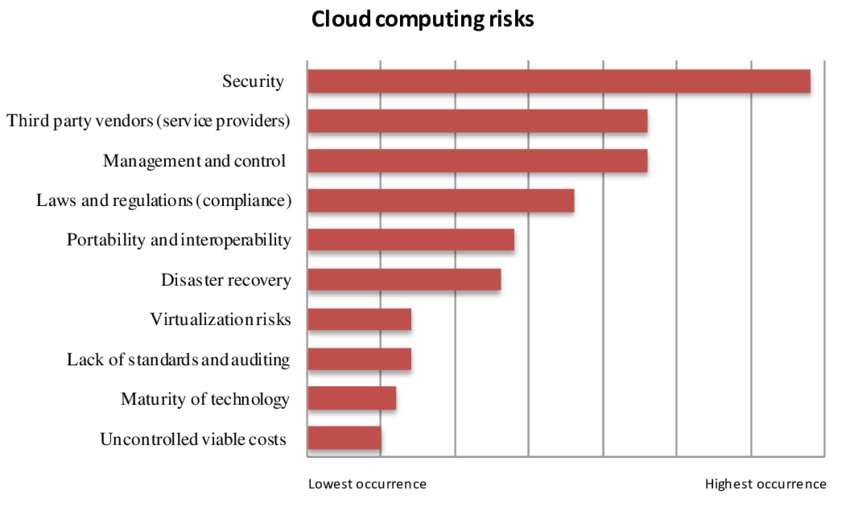
\includegraphics[width=100mm]{images/risks.png}







\section{Μοντέλα υπολογιστικού νέφους}
Ο όρος «Ως Υπηρεσία» \selectlanguage{english}(as a Service), \selectlanguage{greek}αναφέρεται σε μια υπηρεσία Υπολογιστικού Νέφους, η οποία παρέχεται από ένα τρίτο μέρος, με σκοπό να μπορεί ο χρήστης να αφοσιωθεί σε ό,τι έχει περισσότερη σημασία για εκείνον, στην ανάπτυξη ισχυρών και χρήσιμων Πληροφοριακών Συστημάτων και την αύξηση της παραγωγικότητας ή του κέρδους. Ακολουθεί, λοιπόν, μια φιλοσοφία \selectlanguage{english}"Black Box",\selectlanguage{greek} η οποία διευκολύνει το χρήστη και ενθαρρύνει την καινοτομία και τον ανταγωνισμό.

\subsection{Λογισμικό ως Υπηρεσία - \selectlanguage{english}SaaS\selectlanguage{greek}}
Αναμφισβήτητα,η αγορά λογισμικού για τις επιχειρηματικές ανάγκες μιας εταιρείας αποτελεί μια κρίσιμη και περίπλοκη διαδικασία. Στόχος είναι πάντα η ελαχιστοποίηση του κόστους , αλλά και η αύξηση της παραγωγικότητας, επενδύοντας σε όσο μεγαλύτερους αυτοματισμούς. Συνηθισμένα παραδείγματα λογισμικού που χρησιμοποιούνται από τις επιχειρήσεις είναι τα εξής:
\begin{itemize}
  \item Λογισμικό εσωτερικής επικοινωνίας, πχ \selectlanguage{english} Microsoft Teams, Zoom, Webex, Outlook, Jira, Confluence, Slack\selectlanguage{greek}
  \item Λογισμικό για διαχείριση λογιστικών, φορολογικών διαδικασιών
  \item \selectlanguage{english} Enterprise Resource Planning programs (ERP)
  \item Office 365, Word, Excel, Access, Google Docs
  \item Portal \selectlanguage{greek} εταιρείας, διαχείριση αδειών, διαχείριση tickets στο \selectlanguage{english}ΙΤ \selectlanguage{greek}τμήμα \selectlanguage{english}
  \item Version Control System,\selectlanguage{greek} πχ \selectlanguage{english}Github, Gitlab, Bitbucket \selectlanguage{greek}
  \item Λογισμικό διαχείρισης Ανθρωπίνου Δυναμικού \selectlanguage{english}
  \item Customer Relationship Management (CRP), Marketing programs
  \item CAD \selectlanguage{greek}Λογισμικό\selectlanguage{english}
  \item Code Editor,\selectlanguage{greek} πχ\selectlanguage{english} VSCode, IntelliJ, PyCharm\selectlanguage{greek}
\end{itemize}
Παραδοσιακά, αυτή η ανάγκη των εταιρειών ικανοποιούνταν με το λεγόμενο, Λογισμικό ως Προϊόν \selectlanguage{english}(Software as a Product, SaaP), \selectlanguage{greek}βάσει του οποίου, η εταιρεία αγοράζει άδεια για να χρησιμοποιεί τη συγκεκριμένη υπηρεσία, την οποία φιλοξενεί ύστερα, στις εγκαταστάσεις της \selectlanguage{english}(on premises).\selectlanguage{greek} Επίσης, αναλαμβάνει τα έξοδα συντήρησης, ανανέωσης του λογισμικού, τα έξοδα για το υλικό, το ρεύμα, την ασφάλεια. \\ \\
Ωστόσο, με την ανάπτυξη του Υπολογιστικού Νέφους, το Λογισμικό ως Υπηρεσία γίνεται όλο και πιο διαδεδομένο.Το Λογισμικό ως Υπηρεσία, γνωστό και ως \selectlanguage{english}Software as a Service (SaaS) \selectlanguage{greek}αναφέρεται στην παροχή ενός λογισμικού / πληροφοριακού συστήματος, το οποίο φιλοξενείται κεντρικά, στο Νέφος. Η φιλοσοφία πίσω από αυτή τη μέθοδο, είναι πως ο χρήστης μπορεί να απολαμβάνει μια ηλεκτρονική υπηρεσία, χωρίς να χρειάζεται να διαχειρίζεται τις υποδομές, το δίκτυο, τις βάσεις δεδομένων, το ενδιάμεσο λογισμικό, τους διακομιστές / σέρβερς, τα δεδομένα, το λειτουργικό σύστημα, αλλά ούτε και τις εφαρμογές. Εν ολίγοις, ο χρήστης χρησιμοποιεί το Πληροφοριακό Σύστημα , ως συνδρομητής, για να ικανοποιήσει τις ανάγκες του και ο Πάροχος της υπηρεσίας αναλαμβάνει να διαχειρίζεται όλους τους απαιτούμενους πόρους για να λειτουργεί σωστά η εφαρμογή.  \\ 
Τα κυριότερα πλεονεκτήματα ενός τέτοιου μοντέλου είναι τα εξής:
\begin{itemize}
    \itemΧαμηλότερο κόστος για τις επιχειρήσεις και τους ιδιώτες, οι οποίοι δε χρειάζεται να αγοράσουν το λογισμικό και τις απαραίτητες άδειες. Ανάπτυξη οικονομίας κλίμακας με μείωση κόστους συντήρησης και παροχής του λογισμικού. Επίσης, το κόστος είναι συγκεκριμένο \selectlanguage{english}(pay-as-you-go) \selectlanguage{greek}και πολλές φορές δεν υπάρχει από την αρχή της χρήσης (πχ \selectlanguage{english}Netflix).\selectlanguage{greek} 
    \itemΔεν υπάρχει ανάγκη γνώσης χρήσης των διαφόρων λογισμικών, ούτε επομένως και εξειδικευμένου προσωπικού\selectlanguage{english}  (expertise) \selectlanguage{greek} σε μια επιχείρηση, με αποτέλεσμα ξανά τη μείωση κόστους. Ευχρηστία, σύνδεση στην εφαρμογή μέσω κάποιου \selectlanguage{english}Dashboard\selectlanguage{greek} ή \selectlanguage{english}API.\selectlanguage{greek}
    \itemΠρόσβαση από παντού, μέσω Διαδικτύου και οποιασδήποτε συσκευής, χωρίς να χρειάζεται να εγκατασταθεί πρόσθετο λογισμικό (πχ \selectlanguage{english}dependencies,\selectlanguage{greek} εργαλεία, \selectlanguage{english}packages\selectlanguage{greek}, λειτουργικό σύστημα), ή σύνδεση με \selectlanguage{english}VPN\selectlanguage{greek}. Επιτυγχάνεται, λοιπόν, μεγαλύτερη ευελιξία και αύξηση της παραγωγικότητας. Αντίθετα, με τον παραδοσιακό τρόπο απόκτησης ενός λογισμικού από μια εταιρεία, έπρεπε κάποιοι διακομηστές να φιλοξενήσουν την εφαρμογή, καθώς δεν αποτελούσε υπηρεσία Νέφους.
    \itemΌλοι οι χρήστες έχουν την ίδια έκδοση, η οποία αναβαθμίζεται αυτόματα. Έτσι, επιτυγχάνεται καλή συνεργασία μεταξύ των μελών μιας εταιρείας, καθώς υπάρχει συμφωνία και συνοχή (\selectlanguage{english} alignment\selectlanguage{greek}).
    \itemΠρόκειται για ολοκληρωμένα και εύχρηστα Πληροφοριακά Συστήματα, ανεξάρτητα από το Λειτουργικό Σύστημα ή το Υλικό του καθενός, ακολουθούν επομένως τις αρχές της εικονικοποίησης, (\selectlanguage{english}virtualization)\selectlanguage{greek} και της αφαιρετικότητας (\selectlanguage{english}abstraction)\selectlanguage{greek}.
    \itemΚαλύτερη συνεργασία μέσα σε μια εταιρεία, λόγω του \selectlanguage{english}multitenancy,\selectlanguage{greek} δηλαδή της παράλληλης χρήσης της ίδιας εφαρμογής από πολλούς χρήστες. Χαρακτηριστικό του \selectlanguage{english}Multitenancy\selectlanguage{greek} είναι πως οι χρήστες νιώθουν σα να έχουν αποκλειστική χρήση του Λογισμικού και άπειρους πόρους να καταναλώσουν.
    \itemΑσφάλεια από κακόβουλους εισβολείς, προστασία, απόδοση, προσβασιμότητα, υψηλή διαθεσιμότητα, κλιμάκωση, αξιοπιστία και γενικότερα, όλα τα γνωστά πλεονεκτήματα του\selectlanguage{english} Cloud Computing\selectlanguage{greek}. Καθώς οι διάφορες εφαρμογές φιλοξενούνται σε κορυφαία \selectlanguage{english}Data Centers,\selectlanguage{greek} ειδικά σχεδιασμένα με αυτό το σκοπό, σε υψηλού επιπέδου υποδομές, με \selectlanguage{english}firewalls,\selectlanguage{greek} κρυπτογράφηση και ελεγχόμενη πρόσβαση . Οποιοδήποτε πρόβλημα και αν προκύψει, αντιμετωπίζεται εκεί, καθώς διατίθενται άφθονοι πόροι, υπολογισμένοι εκ των προτέρων και βάσει αλγορίθμων και ο χρήστης δε χρειάζεται να ασχοληθεί καθόλου με αυτή τη διαδικασία.
    \itemΧρησιμοποιώντας \selectlanguage{english}SaaS, \selectlanguage{greek}μια επιχείρηση έχει την ευκαιρία να αφοσιωθεί σε αυτό που την ενδιαφέρει πιο πολύ, την ποιότητα του προϊόντος της. Το ίδιο βέβαια ισχύει και για τους ιδιώτες. Αύξηση, λοιπόν, της καινοτομίας και της ευκινησίας \selectlanguage{english}(agility).
\selectlanguage{greek}
\item Οι εταιρείες – πάροχοι εξαρτώνται από την απόφαση των εταιρειών – πελατών να ανανεώσουν το συμβόλαιο μαζί τους , με αποτέλεσμα να υπάρχει ανταγωνισμός και προσπάθεια για διαρκή βελτίωση του λογισμικού που παρέχουν.
\end{itemize} 
Τα κυριότερα μειονεκτήματα του μοντέλου:
\begin{itemize}
 \itemΑναγκαία η χρήση Διαδικτύου, διαφορετικά δεν μπορεί να υπάρξει πρόσβαση στην εφαρμογή . Αντίθετα , με τον παραδοσιακό τρόπο του Λογισμικού ως Προϊόν , σε ορισμένες περιπτώσεις , ήταν εφικτό να γίνεται χρήση της εφαρμογής και χωρίς σύνδεση στο Διαδίκτυο . 
\itemΧαμηλή ασφάλεια ευαίσθητων δεδομένων, αν δεν είναι έμπιστος ο πάροχος.
\itemΈλλειψη ελέγχου, καθώς η υπηρεσία είναι έτοιμη για χρήση και δεν είναι εύκολο να μεταβληθεί και να προσαρμοστεί στις ανάγκες του κάθε χρήστη.
\itemΧαμηλή ταχύτητα μετάδοσης της εφαρμογής, καθώς ο σέρβερ μπορεί να βρίσκεται σε μεγάλη απόσταση από το \selectlanguage{english}Browser, \selectlanguage{greek}όπου τη χρησιμοποιεί ο χρήστης. Για αυτό είναι αναγκαία η επένδυση σε γρήγορη ταχύτητα Διαδικτύου.
\item Δυσκολία συμμόρφωσης με τους κανονισμούς της κυβέρνησης για τα προσωπικά δεδομένα. Η κάθε επιχείρηση θα πρέπει να ενημερωθεί κατάλληλα για τις υποχρεώσεις της.
\item Η εταιρεία δεν αγοράζει στην ουσία το λογισμικό, αλλά το ενοικιάζει, οπότε δε της ανήκει. Αν η εταιρεία που παρέχει την υπηρεσία χρεοκοπήσει για παράδειγμα, η εταιρεία - πελάτης θα αναγκαστεί να αποχωριστεί την υπηρεσία, το οποίο προκαλεί αναστάτωση σε μια μεγάλη επιχείρηση που έχει ανάγκη από σταθερότητα.

\end{itemize}
Συμπέρασμα: \\ \\
Με τη σωστή επιλογή ενός γνωστού και αποδεκτού παρόχου υπηρεσιών λογισμικού, την υπογραφή Συμφωνητικού για το Επίπεδο Λειτουργίας Υπηρεσίας,\selectlanguage{english} SLA (service level agreement),\selectlanguage{greek} όπου καταγράφονται όλες οι νομικές υποχρεώσεις του παρόχου, καθώς και με τη χρήση\selectlanguage{english}  5G,\selectlanguage{greek} το Λογισμικό ως Υπηρεσία είναι μια φτηνή και σίγουρη επιλογή για μια επιχείρηση, ειδικά αν δεν αναζητά κάποια εξειδικευμένη υπηρεσία, όπου έχει ανάγκη\selectlanguage{english}  customization.\selectlanguage{greek}

\subsection{Πλατφόρμα ως Υπηρεσία - \selectlanguage{english}PaaS\selectlanguage{greek}}
Το μοντέλο Πλατφόρμα ως Υπηρεσία \selectlanguage{english}(PaaS)\selectlanguage{greek} παρέχει εργαλεία ανάπτυξης λογισμικού, διεπαφές προγραμματισμού εφαρμογών, έτοιμες υπηρεσίες με σκοπό να υποστηρίξει και να διευκολύνει όλο τον κύκλο της ανάπτυξης λογισμικού\selectlanguage{english} (building, testing, deployment, managing, updating).\selectlanguage{greek} \\
Επιπρόσθετα, ως βασισμένη στο Νέφος υπηρεσία, επιτρέπει στους χρήστες να επωφελούνται από τις υποδομές, το δίκτυο, το λειτουργικό σύστημα, τις βάσεις δεδομένων, τα οποία διαχειρίζεται και συντηρεί ο πάροχος της υπηρεσίας και ταυτόχρονα να έχουν την ευελιξία να σχεδιάσουν και να υλοποιήσουν ο,τιδήποτε επιθυμούν για την επιχείρησή τους, χρησιμοποιώντας έτοιμες μικρο-υπηρεσίες που υπάρχουν ήδη στο περιβάλλον της πλατφόρμας. Διατίθεται μέσω \selectlanguage{english} public, private \selectlanguage{greek}και \selectlanguage{english}hybrid\selectlanguage{greek} νέφους. \\
Παραδείγματα της Πλατφόρμας ως Υπηρεσία:
\begin{itemize}
\item Πλατφόρμα Επικοινωνίας ως Υπηρεσία, \selectlanguage{english}Communications Platform as a Service    (CPaaS) \selectlanguage{greek},η οποία περιλαμβάνει συνδυασμό ήχου, βίντεο, μηνυμάτων και ως στόχο έχει να βελτιώσει τα κανάλια επικοινωνίας μέσα σε μια εταιρεία, πχ \selectlanguage{english}Skype, WhatsApp.
\selectlanguage{greek}Προσφέρει πολλά πλεονεκτήματα στις εταιρείες, καθώς κερδίζουν χρόνο και χρήμα, αφού πλέον δε χρειάζεται να επενδύσουν στην ανάπτυξη δικών τους λύσεων.
\item \selectlanguage{english}Mobile Platform as a Service, \selectlanguage{greek}για την εύκολη ανάπτυξη εφαρμογών, παρέχει έτοιμο κώδικα, με αναλυτικό και βοηθητικό \selectlanguage{english}Documentation, Interactive Development Environment (IDE), Software Development Kit (SDK), run-time\selectlanguage{greek} βιβλιοθήκες για την ανάπτυξη εφαρμογών, ένα ολοκληρωμένο \selectlanguage{english}framework \selectlanguage{greek}ανάπτυξης λογισμικού\selectlanguage{english}.
\item Open PaaS, open source / \selectlanguage{greek}ανοιχτού κώδικα πλατφόρμα, όπου ο χρήστης μπορεί να αναπτύξει εφαρμογές, πολλές φορές με οποιαδήποτε γλώσσα προγραμματισμού ή βάση δεδομένων επιθυμεί πχ \selectlanguage{english}Google App Engine, Microsoft Azure, Heroku\selectlanguage{greek}.
\itemΜια άλλη αξιοσημείωτη χρήση  \selectlanguage{english}PaaS \selectlanguage{greek}είναι στα \selectlanguage{english}DevOps tools (CI/CD pipelines), \selectlanguage{greek}τα οποία βοηθούν στην ανάπυξη και διατήρηση λογισμικού (πχ \selectlanguage{english}Azure DevOps).
\item Integrations PaaS (iPaas) \selectlanguage{greek}για συγχώνευση δεδομένων, υπηρεσιών κτλ που βρίσκονται σε διαφορετικά περιβάλλοντα πχ στο Νέφος και τοπικά. Προσφέρουν εύκολη χρήση, ευελιξία, αποδοτικότητα και ταχύτητα. Παραδείγματα αυτής της υπηρεσίας είναι για συγχώνευση εφαρμογών, \selectlanguage{english}microservices (API),\selectlanguage{greek} πλατφορμών, συσκευών \selectlanguage{english}IoT (Internet of Things)\selectlanguage{greek} κτλ\selectlanguage{english}.
\item \selectlanguage{english}AIPaaS, \selectlanguage{greek}για δημιουργία μοντέλων Μηχανικής Μάθησης με προεκπαιδευμένα/\selectlanguage{english}pre-trained\selectlanguage{greek} μοντέλα (αναγνώριση ομιλίας, εικόνας, κατηγοριοποίηση). Η ανάπτυξη του Υπολογιστικού Νέφους καθιστά δυνατή την διαχείριση, ανάλυση και υπολογισμό μεγάλου όγκου δεδομένων , με απότελεσμα να είναι εφικτή η δημιουργία έξυπνων εφαρμογών που κάνουν προβλέψεις και αυξάνουν την αυτοματοποίηση και την αποδοτικότητα των εταιρειών. Επίσης, χάρη στο \selectlanguage{english}AIPaaS, \selectlanguage{greek}οι \selectlanguage{english}Data Scientists \selectlanguage{greek}μπορούν να αφοσιωθούν στην περίπλοκη δουλειά τους, αντί να ασχολούνται με τις δυσκολίες και τις προκλήσεις των υποδομών.
\item Η Πλατφόρμα ως Υπηρεσία κυριαρχεί στην τεχνολογία του \selectlanguage{english}IoT ( Internet of Things ),\selectlanguage{greek} καθώς προσφέρει οικονομική αποθήκευση δεδομέων στο Νέφος, ασφάλεια, φιλτράρισμα και ανάλυση των πληροφοριών, διαχείριση των συσκευών, προσβασιμότητα από παντού, ταχύτητα , δυνατότητα διαχείρισης δικτυακής σύνδεσης και αυτοματοποίηση διαδικασιών. Για αυτό και οι μεγάλοι πάροχοι Νέφους προσφέρουν ειδικές υπηρεσίες για\selectlanguage{english} IoT (eg AWS IoT)\selectlanguage{greek}.
\end{itemize}
Τα κυριότερα πλεονεκτήματα ενός τέτοιου μοντέλου είναι τα εξής :
\begin{itemize}
\item Οι προγραμματιστές μπορούν να αφοσιωθούν στην ανάπτυξη λογισμικού και συγκεκριμένα στη λογική \selectlanguage{english}(business intelligence)\selectlanguage{greek} πίσω από την εκάστοτε εφαρμογή, αντί να χάνουν χρόνο με την υποδομή, το δίκτυο, το λειτουργικό σύστημα, την αποθήκευση, τους διακομιστές. Όλα αυτά τα αναλαμβάνει ο πάροχος. Μείωση, λοιπόν, του \selectlanguage{english}low level  programming,\selectlanguage{greek} το οποίο είναι και το πιο απαιτητικό και εξοικονόμηση χρόνου.
\item Απλό μοντέλο, χαμηλό κόστος για ανάπτυξη εφαρμογών, καθώς δεν υπάρχει ανάγκη για εγκατάσταση και συντήρηση υποδομών ή λειτουργικού συστήματος \selectlanguage{english} (pay-as-you-go)\selectlanguage{greek}.
\item Προσβασιμότητα, υψηλή διαθεσιμότητα, κλιμάκωση, καθώς γίνεται χρήση πόρων με βάση τη ζήτηση, τους οποίους τους παρέχει ο Πάροχος.
\item Μείωση απαιτούμενου κώδικα, καθώς παρέχονται έτοιμα πολλά χρήσιμα εργαλεία \selectlanguage{english}(pre-coded components, sample code, software tools, kits, libraries), \selectlanguage{greek}αύξηση της παραγωγικότητας.
\item Εύκολη μεταφορά στο Υβριδικό Νέφος.
\item Έτοιμο περιβάλλον για \selectlanguage{english}versioning, build (debugger, compiler, code editor), deployment, testing, monitoring,\selectlanguage{greek} διαθέσιμα\selectlanguage{english} plugins\selectlanguage{greek} και \selectlanguage{english}frameworks\selectlanguage{greek} που διευκολύνουν αισθητά τη χρήση της πλατφόρμας. Επιπρόσθετα,  το μοντέλο \selectlanguage{english}PaaS \selectlanguage{greek}παρέχει συχνά εργαλεία για\selectlanguage{english} Data Analytics, \selectlanguage{greek}για δεδομένα που αφορούν το χρήστη ως προς την εφαρμογή.
\item Παροχή ενσωματωμένης βάσης \selectlanguage{english}(Database as a Service, \selectlanguage{greek}πχ \selectlanguage{english}MongoDB Atlas)\selectlanguage{greek},και γενικότερα έτοιμων και εύχρηστων υπηρεσιών.
\item Παρέχει τα θετικά του \selectlanguage{english}SaaS, \selectlanguage{greek}όσον αφορά την ανεξαρτησία από τις υποδομές, αλλά προσφέρει ακόμη και επιπλέον ευελιξία, καθώς ο χρήστης μπορεί να δημιουργήσει ο,τιδήποτε επιθυμεί για να καλύψει πλήρως τις ανάγκες του, κάτι που ίσως δε θα μπορούσε να γίνει με ένα\selectlanguage{english} SaaS,\selectlanguage{greek} το οποίο δίνεται έτοιμο.
\item Παρόμοιο μοντέλο με το Συνάρτηση ως Υπηρεσία\selectlanguage{english} (Function as a Service), Serverless as a Service,\selectlanguage{greek} όπου σημασία έχει η λογική και όχι και η υποδομή
\end{itemize}
Τα κυριότερα μειονεκτήματα του μοντέλου:
\begin{itemize}
\item Δύσκολη μετακίνηση σε άλλο πάροχο, καθώς είναι πιθανό εκεί να γίνονται με άλλον τρόπο οι διαδικασίες ή να μην παρέχονται οι ίδιες υπηρεσίες/ευκολίες κτλ\selectlanguage{english} (Vendor lock-in)\selectlanguage{greek}
\item Εξάρτηση από τον πάροχο, η τιμή μπορεί να αυξηθεί ανά πάσα στιγμή, αν υπάρξει πρόβλημα στις υποδομές, η εφαρμογή θα καταρρεύσει
\item Έλλειψη ελέγχου, όπως και στο μοντέλο Λογισμικό ως Υπηρεσία, καθώς κάποιος άλλος καθορίζει μεγάλο μέρος των \selectlanguage{english}configurations
\selectlanguage{greek}
\item Κίνδυνος κλοπής δεδομένων εταιρείας, καθώς τα διαχειρίζεται κάποιος τρίτος
\end{itemize}
Συμπέρασμα: \\ \\
Με τη σωστή επιλογή της υπηρεσίας, ώστε να καλύπτει τις ανάγκες της επιχείρησης/του χρήστη, αλλά και να ανήκει σε έμπιστο πάροχο, η Πλατφόρμα ως Υπηρεσία μπορεί να βελτιώσει και να διευκολύνει τη δουλειά του \selectlanguage{english}Developer, \selectlanguage{greek}καθώς δε χρειάζεται να ξεκινάει από το μηδέν για κάθε του εργασία.

\subsection{Υποδομή ως Υπηρεσία -\selectlanguage{english} IaaS\selectlanguage{greek}}
Πρόκειται για ένα μοντέλο με το οποίο ο χρήστης/η επιχείρηση ενοικιάζεται και διαχειρίζεται, παρακολουθεί, αυξομειώνει πόρους \selectlanguage{english}(resources)\selectlanguage{greek}, μνήμη,\selectlanguage{english} CPU, \selectlanguage{greek}σέρβερς, βάσεις δεδομένων \selectlanguage{english}(replicas),\selectlanguage{greek} δικτυακό εξοπλισμό, τα οποία δε βρίσκονται στις τοπικές εγκαταστάσεις \selectlanguage{english}(on premises),\selectlanguage{greek} αλλά φιλοξενούνται στο\selectlanguage{english} cloud, \selectlanguage{greek}δηλαδή σε κάποιο \selectlanguage{english}Data Center.\selectlanguage{greek} Το όφελος αυτού του μοντέλου, και συνεπώς και των προαναφερθέντων, είναι ασύλληπτο, και οικονομικά αλλά και από άποψη χρόνου, προσπάθειας και ασφάλειας. \\ \\
Τα πιο γνωστά παραδείγματα \selectlanguage{english}IaaS:
\begin{itemize}
\item AWS (Amazon Web Services) EC2, 
\item Microsoft Azure, 
\item Google Cloud Platform, 
\item IBM Cloud, 
\item Oracle Cloud
\end{itemize}
\selectlanguage{greek}
Συγκεκριμένα τα πλεονεκτήματα είναι τα εξής : 
\begin{itemize}
\item Eλαχιστοποιείται το κόστος της κτήσης και συντήρησης της υλικοτεχνικής υποδομής \selectlanguage{english}(hardware),\selectlanguage{greek} μέσω της εικονικοποιήσης \selectlanguage{english}(virtualization), \selectlanguage{greek}διότι δεν υπάρχει ανάγκη για αγορά νέου εξοπλισμού. Ακόμα και για μια μικρή \selectlanguage{english}start-up\selectlanguage{greek} εταιρεία υπάρχει συμφέρον  στη μίσθωση υποδομών ως υπηρεσία.
\item Μπορεί εύκολα να επιτευχθεί κλιμάκωση και υψηλή διαθεσιμότητα\selectlanguage{english}(high availability), \selectlanguage{greek}μέσω διάφορων μεθόδων που συμφωνούνται στο\selectlanguage{english} SLA.\selectlanguage{greek} Έτσι, αν πχ τεθεί ένα όριο/threshold που αφορά την χρήση των πόρων, και το υπερβούμε, τότε αυτόματα και χωρίς καθυστέρηση θα μπουν σε χρήση νέοι πόροι. Επιπλέον, αν χρειαζόμαστε λιγότερους πόρους  απ’ ότι χρησιμοποιούσαμε μέχρι τώρα, μπορούμε πάλι εύκολα να κάνουμε \selectlanguage{english}scale down/in, \selectlanguage{greek}και να μειώσουμε το κόστος. Διαφορετικά, αν αυτές οι ενέργειες γίνοταν στις εγκαταστάσεις της εταιρείας, οι σέρβερς που είχαμε αγοράσει, θα έμεναν άπραγοι.
\item Λόγω του\selectlanguage{english} load balancing \selectlanguage{greek}που γίνεται με μικρό κόστος, αποφεύγεται το \selectlanguage{english}single point of failure,\selectlanguage{greek} δηλαδή η περίπτωση, αν κάτι δε δουλέψει σωστά, να καταρρεύσει όλη η εφαρμογή. Στο Νέφος, η εφαρμογή, τα δεδομένα, οι βάσεις δεδομένων βρίσκονται ταυτόχρονα σε πολλά σημεία, ακόμα και γεωγραφικά, ώστε να μην υπάρχει κανένας φόβος για τέτοιο ενδεχόμενο \selectlanguage{english}(availability zones).\selectlanguage{greek}
Στο \selectlanguage{english}IaaS, \selectlanguage{greek}λοιπόν, οι πόροι χρησιμοποιούνται ανάλογα με τη ζήτηση \selectlanguage{english}(on demand).\selectlanguage{greek}
\item Το \selectlanguage{english}IaaS \selectlanguage{greek}προσφέρει ασφάλεια, καθώς οι χρήστες που έχουν πρόσβαση στους διακομιστές και άλλα σημαντικά συστήματα φιλτράρονται.
\item Προσβασιμότητα από παντού, μέσω \selectlanguage{english}Web 2.0\selectlanguage{greek}
\item Λόγω της δύναμης των παρόχων στην αγορά, οι υποδομές που διατίθενται είναι κορυφαίας τεχνολογίας αλλά και επιλεγμένες για την κάθε ξεχωριστή περίπτωση και για τις ανάγκες του κάθε πελάτη. Επίσης, καθιστούν δυνατή την επεξεργασία \selectlanguage{english}Big Data, \selectlanguage{greek}κάτι που προφανώς είναι απαραίτητο στη σύγχρονη εποχή
\item Το πιο ευέλικτο μοντέλο, ο χρήστης έχει πλήρη έλεγχο πάνω στις υποδομές\selectlanguage{english} (abstraction)\selectlanguage{greek}
\item Πολλοί χρήστες χρησιμοποιούν το ίδιο \selectlanguage{english}hardware (multitenancy)\selectlanguage{greek}
\item Μια επιχείρηση μπορεί να έχει πρόσβαση σε σέρβερς που βρίσκονται γεωγραφικά κοντά στους χρήστες της εφαρμογής, με αποτέλεσμα να μεταδίδεται με καλύτερη ταχύτητα το προϊόν.
\end{itemize}
 Τα κυριότερα μειονεκτήματα του μοντέλου:
\begin{itemize}
\item Πάντα υπάρχει η ανησυχία για την ασφάλεια των δεδομένων, ειδικά λόγω του\selectlanguage{english} multitenancy. \selectlanguage{greek}Πρέπει κανείς να σιγουρευτεί πως τα δεδομένα του είναι απομονωμένα από τους άλλους χρήστες
\item Αν κάποιος δε ξέρει να χειρίζεται σωστά τις υπηρεσίες του \selectlanguage{english}Cloud Provider,\selectlanguage{greek} υπάρχει ο κίνδυνος να κάνει λάθη που να του κοστίσουν ακριβά, ενώ στην περίπτωση πχ του\selectlanguage{english} SaaS \selectlanguage{greek}δεν υπάρχει αυτός ο κίνδυνος.
\end{itemize}
Ένα παρόμοιο και αξιοσημείωτο μοντέλο υπηρεσίας είναι το\selectlanguage{english} Bare-Metal as a Service (BMaaS),\selectlanguage{greek} με το οποίο ο χρήστης έχει άμεση πρόσβαση στο υλικό πίσω από την εφαρμογή του, και όχι σε μια εικονοποιημένη μορφή του, με αποτέλεσμα να έχει καλύτερο έλεγχο αλλά να του κοστίζει σε χρόνο. \\ \\
Συμπέρασμα: \\ \\
Όταν μια εταιρεία περιμένει μεγάλη ανάπτυξη, την οποία και δε μπορεί να προβλέψει ακριβώς, θα επωφεληθεί ιδιαιτέρως από τέτοιου είδους αυτοματισμούς στο υλικό.Ωστόσο, είναι σημαντικό για μια εταιρεία να έχει εξειδικευμένο προσωπικό που να ξέρει να παρακολουθεί τη χρήση των πόρων \selectlanguage{english}(monitoring), \selectlanguage{greek}να συμβουλεύεται\selectlanguage{english} Cloud Solutions Architects,\selectlanguage{greek} ώστε να χρησιμοποιεί πάντα τις πιο αποδοτικές υπηρεσίες, να παρακολουθεί το \selectlanguage{english}billing \selectlanguage{greek}και να θέτει\selectlanguage{english} thresholds \selectlanguage{greek}και\selectlanguage{english} alerts, \selectlanguage{greek}για να αποφύγει παραβιάσεις στην κατανάλωση των πόρων.


\subsection{Συνάρτηση ως Υπηρεσία - \selectlanguage{english}FaaS\selectlanguage{greek}}
Το μοντέλο \selectlanguage{english}Function as a Service, \selectlanguage{greek}το οποίο ανήκει στην ευρύτερη οικογένεια των \selectlanguage{english}“Serverless” \selectlanguage{greek}μοντέλων (πολλές φορές λανθασμένα ταυτίζονται), αποτελεί μια νέα σχετικά εξέλιξη καθώς πρωτοεμφανίστηκε στις αρχές της δεκαετίας του 2010, με την πρώτη μεγάλη εταιρία του χώρου που προσέφερε την υπηρεσία αυτή να είναι η \selectlanguage{english}Amazon\selectlanguage{greek} με το \selectlanguage{english}AWS Lambda \selectlanguage{greek}το 2014. Το μοντέλο αυτό στοχεύει στην απλοποίηση της σχεδίασης και της εκτέλεσης λογισμικού στο Υπολογιστικό Νέφος \selectlanguage{english}(Cloud)\selectlanguage{greek}, μέσα από την ανάθεση στον πάροχο της εκτέλεσης αυτοτελών τμημάτων κώδικα που εκτελούνται με έναυσμα κάποιο γεγονός τα οποία ονομάζονται Συναρτήσεις \selectlanguage{english}(Functions).\selectlanguage{greek} Η λογική των Συναρτήσεων αποτελεί ουσιαστικά επέκταση της αρχιτεκτονικής των \selectlanguage{english}Microservices, \selectlanguage{greek}όπου μια εφαρμογή υλοποιείται ως σύνολο μικρότερων, ημιαυτόνομων υπηρεσιών, που επικοινωνούν η μια με την άλλη μέσω διεπαφών. Η εφαρμογή έτσι φιλοξενείται σε διακομιστή του παρόχου, και όταν λόγω κάποιου γεγονότος, για παράδειγμα κάποιας δραστηριότητας ενός χρήστη, απαιτηθεί η εκτέλεση κάποιας Συνάρτησης, αυτή ανατίθεται στις υποδομές του παρόχου, που ενεργοποιούνται, την εκτελούν και έπειτα αδρανοποιούνται μετά την ολοκλήρωση της για λόγους οικονομίας. 

Μερικοί από τους πιο δημοφιλείς παρόχους είναι οι εξής:
\selectlanguage{english}
\begin{itemize}
\item AWS Lambda
\item Azure Cloud Functions
\item Google Cloud Functions
\item Oracle Functions
\item IBM Functions
\item Cloudflare Workers
\end{itemize}
\selectlanguage{greek}
Ας εξετάσουμε τα κυριότερα πλεονεκτήματα της χρήσης \selectlanguage{english}Function as a Service:
\selectlanguage{greek}

\begin{itemize}
\item Οι υποδομές του παρόχου απασχολούνται, και επομένως αυτός χρεώνει τον οργανισμό/ πελάτη μόνο κατά την εκτέλεση μια συνάρτησης. Έτσι, ο οργανισμός/ πελάτης δεν συσσωρεύει έξοδα σε περιόδους αδράνειας, καθώς πληρώνει μόνο βάσει του συνολικού χρόνου εκτελέσεων. Επιπλέον, τα έξοδα αγοράς, αναβάθμισης, συντήρησης διακομιστών και άλλες δαπάνες βαραίνουν μόνο τον πάροχο, έτσι το μοντέλο είναι ιδιαίτερα συμφέρον για οργανισμούς που έχουν περιορισμένες ανάγκες και επομένως η αγορά και συντήρηση ιδιόκτητων διακομιστών δεν θα ήταν συμφέρουσα.
\item Ενισχύεται η επεκτασιμότητα του λογισμικού, μιας και οι πάροχοι έχουν την δυνατότητα να διανείμουν στο δίκτυο των διακομιστών τους τυχόν αυξημένο φόρτο από αιτήματα του πελάτη, δεσμεύοντας και αποδεσμεύοντας τις υποδομές τους με τον κατάλληλο τρόπο ώστε να ικανοποιήσουν τα αιτήματα του πελάτη στο μικρότερο δυνατό χρονικό διάστημα. Καθώς το μοντέλο\selectlanguage{english} Function as a Service \selectlanguage{greek}ακολουθεί την λογική των \selectlanguage{english} Microservices, \selectlanguage{greek}προσφέρει εγγενώς μεγαλύτερες δυνατότητες επεκτασιμότητας σε σχέση με μονολιθικές αρχιτεκτονικές, ακόμα και αν οι δεύτερες φιλοξενούνται στο Υπολογιστικό Νέφος. Για τον ίδιο λόγο είναι και ευκολότερο το τεστάρισμα τέτοιων εφαρμογών.
\item Καθώς η εφαρμογή υλοποιείται ως σύνολο απλών και σε μεγάλο βαθμό αυτοτελών τμημάτων κώδικα, είναι αποτελεσματική η ανάπτυξη της εφαρμογής από διαφορετικές ομάδες, αυξάνοντας της ταχύτητα υλοποίησης και μειώνοντας τον χρόνο που απαιτείται από τον αρχικό σχεδιασμό μέχρι την παράδοση του προϊόντος/ υπηρεσίας. Ακόμα, τα μικρότερα αυτοτελή τμήματα κώδικα είναι ιδανικά για τη μέθοδο Συνεχούς Ανάπτυξης \selectlanguage{english}(Iterative Development), \selectlanguage{greek}μιας και μπορούν εύκολα και γρήγορα να γίνουν αλλαγές σε αυτά ακόμα, και παράλληλα, επιταχύνοντας σημαντικά την όλη διαδικασία.
\end{itemize}

Υπάρχουν όμως και κάποια σημαντικά ελαττώματα του μοντέλου που πρέπει ο οργανισμός να σταθμίσει με τα παραπάνω προτερήματα:

\begin{itemize}
\item Όπως και σε άλλα μοντέλα που βασίζονται στο Υπολογιστικό Νέφος είναι υπαρκτός ο κίνδυνος να παγιδευτεί ο πελάτης από την εξάρτηση του στις υπηρεσίες που παρέχει ο συγκεκριμένος πάροχος με τρόπο που καθιστά δύσκολη την αλλαγή παρόχου σε περίπτωση που αυτό κριθεί απαραίτητο λόγω για παράδειγμα αύξησης της τιμής από τον τρέχων πάροχο. Αυτό μπορεί να προσφέρει την δυνατότητα στον παρόχο να αυξήσει τις τιμές, καθώς αποκτά αυξημένη διαπραγματευτική ισχύ πάνω στους υπάρχοντες πελάτες του. Το μοντέλο \selectlanguage{english}FaaS \selectlanguage{greek}αντιμετωπίζει το πρόβλημα αυτό αλλά σε κάθε περίπτωση σε πιο ήπιο βαθμό σε σχέση με μοντέλα όπως το  \selectlanguage{english}Backend as a Service,  \selectlanguage{greek}που η λειτουργικότητα βασίζεται εξ' ολοκλήρου στον πάροχο και έτσι η υλοποίηση του λογισμικού πρέπει να αλλάξει ριζικά, ενώ στο υπό εξέταση μοντέλο ο πελάτης μπορεί να μεταφέρει τον κώδικα ως έχει ή με μικρές αλλαγές.
\item Για την εκτέλεση μιας συνάρτησης, ο πάροχος ενδέχεται μέσα από το σύστημα διαχείρισης των πόρων του να ενεργοποιήσει κάποιον αδρανή διακομιστή. Αυτή η διαδικασία, καθώς και άλλες δραστηριότητες που σχετίζονται με την ανάθεση Συναρτήσεων στις υποδομές του παρόχου ενδέχεται να δημιουργήσουν καθυστερήσεις αυξάνοντας τον συνολικό χρόνο απόκρισης της εφαρμογής.
\item Λόγω του μοντέλου χρέωσης με βάση την χρήση \selectlanguage{english}(Pay as you Go) \selectlanguage{greek}είναι υπαρκτός ο κίνδυνος μια εφαρμογή να πέσει θύμα επιθέσεων, κατά τις οποίες οι επιτιθέμενοι, υποδυόμενοι τους καλοπροαίρετους χρήστες, δημιουργούν την ανάγκη εξυπηρέτησης μεγάλου αριθμού αιτημάτων, με στόχο να προκαλέσουν οικονομική ζημία στον οργανισμό που θα πληρώσει για την διεκπεραίωσή τους. Οι πάροχοι προσφέρουν μεθόδους καταπολέμησης τέτοιων επιθέσεων, μειόνοντας ή σταματώντας εξ' ολοκλήρου την εκτέλεση αιτημάτων σε περίπτωση που αυτά αρχίσουν να γίνονται με ταχύτητα μεγαλύτερη από ένα όριο το οποίο θεωρείται το φυσιολογικό. Έτσι όμως προκύπτει ζήτημα σχετικά με την κλιμάκωση, καθώς στο όνομα της προστασίας περιορίζεται η δυνατότητα της εφαρμογής να ανταποκριθεί σε περιπτώσεις πραγματικής ραγδαία αυξανόμενης ζήτησης αν τέτοιες προκύψουν.
\item Τέλος, αρκετοί πάροχοι επιβάλλουν όρια στην διαδικασία εκτέλεσης των συναρτήσεων, σχετιζόμενα με τον χρόνο εκτέλεσης, την ποσότητα μνήμης που επιτρέπεται σε μία ή το σύνολο τον συναρτήσεων να καταναλώσουν ή και άλλους περιορισμούς. Για παράδειγμα, στην \selectlanguage{english}AWS Lambda, \selectlanguage{greek}ο μέγιστος χρόνος εκτέλεσης περιορίζεται στα 300\selectlanguage{english}ms, \selectlanguage{greek}και η μέγιστη μνήμη στα 1500\selectlanguage{english}mb\selectlanguage{greek}, ενώ στην πλατφόρμα \selectlanguage{english}Google Cloud\selectlanguage{greek} περιορίζεται στα 500\selectlanguage{english}ms\selectlanguage{greek}. Επομένως ενδέχεται το \selectlanguage{english}FaaS\selectlanguage{greek} να μην είναι η ιδανική λύση αν ο χρόνος εκτέλεσης τμήματος της εφαρμογής είναι πιθανό να ξεπεράσει αυτά τα όρια. 
\end{itemize}


\subsection {Σύστημα Υποστήριξης ως Υπηρεσία - \selectlanguage{english}BaaS}\selectlanguage{greek}
Πρόκειται για ένα μοντέλο βάσει του οποίου ο οργανισμός/χρήστης αναλαμβάνει να υλοποιήσει και να συντηρεί μόνο το ορατό από τον τελικό χρήστη μέρος της εφαρμογής \selectlanguage{english}(Frontend),\selectlanguage{greek} καθώς όλες τις υποστηρικτικές υπηρεσίες \selectlanguage{english}(Backend) \selectlanguage{greek}αναλαμβάνει να προσφέρει ο πάροχος. Ο οργανισμός/χρήστης αυτού του μοντέλου μπορεί αφενός να αφοσιωθεί στον σχεδιασμό της εμπειρίας του τελικού χρήστη, λαμβάνοντας άλλες υποστηρικτικές υπηρεσίες όπως βάσεις δεδομένων, την διαδικασία σύνδεσης και αυθεντικοποίησης του χρήστη, την φιλοξενία του λογισμικού σε κάποιον διακομιστή και άλλα επιμέρους ζητήματα υλοποίησης ως δεδομένα, εξοικονομώντας χρόνο και χρήμα. Το μοντέλο αυτό συναντάται και ως \selectlanguage{english}Mobile Backend as a Service (MBaaS), \selectlanguage{greek}καθώς συχνά χρησιμοποιείται σε εφαρμογές κινητών τηλεφώνων, γενικά όμως οι δύο ονομασίες αναφέρονται στο ίδιο μοντέλο.

Μερικοί από τους πιο δημοφιλείς παρόχους είναι:
\begin{itemize}
\selectlanguage{english}
\item Apache Usergrid
\item Amazon Web Services (AWS) Amplify
\item Back4App
\item Firebase
\item MongoDb Stitch
\end{itemize}
\selectlanguage{greek}
Η χρήση του μοντέλου \selectlanguage{english}Backend as a Service \selectlanguage{greek}προσφέρει κάποια σημαντικά πλεονεκτήματα:
\begin{itemize}
\item Αυξημένη ταχύτητα ανάπτυξης, καθώς ο οργανισμός αποφεύγει την υλοποίηση των πιο πολύπλοκων στην σχεδίαση και χρονοβόρων στην υλοποίηση τμημάτων της εφαρμογής, τα οποία μπορεί να λάβει ως δεδομένα, αφού τα προσφέρει ο πάροχος, και να χρησιμοποιήσει μέσω απλών στην χρήση διεπαφών προγραμματισμού εφαρμογών (\selectlanguage{english}API’s\selectlanguage{greek}), χωρίς να χρειάζεται να τα σχεδιάσει από την αρχή.
\item Μειωμένο κόστος κατά τη σχεδίαση, πρώτον λόγω του μειωμένου χρόνου ανάπτυξης καθώς ο οργανισμός θα διανύσει σημαντικά λιγότερο χρόνο από την στιγμή της αρχικής επένδυσης μέχρι την στιγμή που το σύστημα θα είναι έτοιμο για χρήση, επομένως θα μπορέσει να αποσβέσει το όποιο κόστος πρόσκτησης αυτής της υπηρεσίας γρηγορότερα σε σχέση με το χρόνο απόσβεσης στην περίπτωση που το \selectlanguage{english}backend \selectlanguage{greek}από την αρχή. Ο δεύτερος λόγος είναι πως ο οργανισμός αποφεύγει την απασχόληση εξειδικευμένου προσωπικού ή την εξωτερική ανάθεση του έργου της δημιουργίας ενός τέτοιου συστήματος. Το κόστος μειώνεται περαιτέρω κατά τη λειτουργία, αφού ο πάροχος προσφέρει και τις υποδομές πάνω στις οποίες εκτελούνται όλες αυτές οι υπηρεσίες, εξοικονομώντας το κόστος λειτουργίας που θα έπρεπε να καλύψει ο οργανισμός αν οι υποδομές αυτές ήταν ιδιόκτητες, ενώ δεν είναι και απαραίτητη η απασχόληση ειδικά καταρτισμένου προσωπικού που θα επιβλέπει την λειτουργία τόσο των υπηρεσιών όσο και του αντίστοιχου υλικού από τον οργανισμό.
\item Αυξημένη επεκτασιμότητα, μιας και οι διακομιστές στους οποίους πραγματοποιούνται οι \selectlanguage{english}backend \selectlanguage{greek}εργασίες δεν ανήκουν στην επιχείρηση, αλλά στον πάροχο της υπηρεσίας, ο οποίος δεσμεύεται να προσφέρει την κατάλληλη επεξεργαστική ισχύ όπως και όταν αυτή απαιτείται. Έτσι είναι εύκολο και να αυξηθούν οι πόροι που είναι αφοσιωμένοι στην εφαρμογή, ή να μειωθούν αν δεν είναι απαραίτητοι, και καθώς σύμφωνα με την τιμολογιακή πολιτική των περισσοτέρων παρόχων, η χρέωση γίνεται με βάση το πλήθος των πόρων που απασχολούνται και με τον χρόνο που απασχολούνται, ο οργανισμός πληρώνει ακριβώς όσο του είναι απαραίτητο. Σε αντίθετη περίπτωση, εάν δηλαδή ο οργανισμός φιλοξενούσε όλες τις λειτουργίες σε δικές του υποδομές θα ήταν κοστοβόρο και χρονοβόρο να αυξηθεί η υπολογιστική ισχύς (παραγγέλνοντας επιπλέον μηχανήματα για να αναλάβουν το ρόλο διακομιστών για παράδειγμα), ενώ σε περιόδους μειωμένης ζήτησης, η επένδυση του οργανισμού στους επιπλέον πόρους που δεν χρησιμοποιεί τη δεδομένη στιγμή θα πήγαινε χαμένη.
\item Λόγω της κλίμακας στην οποία δραστηριοποιούνται οι εταιρείες πάροχοι, είναι αποτελεσματικό και οικονομικά συμφέρον για αυτές να επενδύσουν στις πιο σύγχρονες μεθόδους ασφάλειας δεδομένων και να εφαρμόσουν όλα τα κατάλληλα πρωτόκολλα, προσφέροντας μεγαλύτερη ασφάλεια από ότι θα μπορούσε ποτέ να προσφέρει ο οργανισμός μόνος του, τουλάχιστον χωρίς να δαπανήσει μεγάλα χρηματικά ποσά και εργατοώρες σε αυτό τον τομέα, σε βαθμό που θα έκανε το όλο εγχείρημα ασύμφορο. Επιπλέον οι πάροχοι αναλαμβάνουν να προσφέρουν τα απαραίτητα πρωτόκολλα ώστε να διευκολύνουν τους οργανισμούς στους οποίους προσφέρουν υπηρεσίες να συμμορφωθούν με το υπάρχον νομικό πλαίσιο προστασίας των προσωπικών δεδομένων, όπως για παράδειγμα με τον νόμο \selectlanguage{english}GDPR\selectlanguage{greek} της Ευρωπαϊκής Ένωσης, κάτι που σε αντίθετη περίπτωση θα απαιτούσε επιπλέον πόρους από τον οργανισμό.
\end{itemize}
Το μοντέλο αυτό όμως παρουσιάζει και κάποια σημαντικά ελαττώματα τα οποία θα δούμε αναλυτικά και αναφέρονται κυρίως στην έλλειψη άμεσου ελέγχου που είναι εγγενής σε αυτού του είδους τα μοντέλα:

\begin{itemize}
\item Αρχικά, οι μέθοδοι που χρησιμοποιεί ο πάροχος για να προσφέρει μια συγκεκριμένη λειτουργικότητα είναι αυτοί που θα αποδίδουν καλύτερα στο μεγαλύτερο ποσοστό των πιθανών προβλημάτων, λόγω του μεγάλου αριθμού οργανισμών που αυτός καλείται να εξυπηρετήσει. Στον κλάδο της πληροφορικής όμως δεν είναι πάντα δυνατό να βρεθεί λύση που να είναι βέλτιστη για κάθε σενάριο χρήσης, και έτσι είναι πιθανό η προσέγγιση που χρησιμοποιεί ο πάροχος για να επιλύσει ένα πρόβλημα να μην είναι η αποδοτικότερη για το είδος του προβλήματος που καλείται να επιλύσει ένας συγκεκριμένος οργανισμός, και καθώς ο τελευταίος τις πιο πολλές φορές δεν έχει κανέναν έλεγχο πάνω στην υλοποίηση, δεν υπάρχει τρόπος να την παραμετροποιήσει  και να το βελτιώσει για τις ανάγκες του.
\item Καθώς όποια εφαρμογή αναπτυχθεί, θα βασίζεται στην αρχιτεκτονική που προσφέρει ο πάροχος μέσω διεπαφών, απαιτείται χρόνος και κατά συνέπεια χρήμα για μεταφορά σε άλλου είδους λύση ή/και διαφορετικο πάροχο, καθώς πρέπει να υπάρξουν αλλαγές στο \selectlanguage{english}Frontend \selectlanguage{greek}κομμάτι της εφαρμογής. Ο πάροχος μπορεί να το εκμεταλλευτεί αυτό σε βάθος χρόνου, για παράδειγμα αυξάνοντας την τιμή.
\item Ένα άλλο ζήτημα που εγείρεται είναι αυτό της αξιοπιστίας ως προς την λειτουργία. Καθώς ο πάροχος είναι συνήθως ιδιωτική εταιρεία, είναι στη σφαίρα του πιθανού για οικονομικούς ή άλλους λόγους που δύσκολα μπορεί να προβλέψει ή να ελέγξει ο οργανισμός, να παύσει την προσφορά υπηρεσιών ή την λειτουργία του γενικότερα. Αυτό δεν περιορίζεται μόνο σε μικρότερους παρόχους που θα περίμενε κανείς να είναι λιγότερο ανταγωνιστικοί λόγω μεγέθους, αλλά μπορεί να προκύψει ακόμα και σε μεγαλύτερες εταιρείες, όπως μας δείχνει το παράδειγμα της πλατφόρμας \selectlanguage{english}Parse\selectlanguage{greek}. Η πλατφόρμα αυτή αποτελούσε μια απο τις πιο δημοφιλείς στον κλάδο και κάλυπτε μεγάλο μέρος της αγοράς, έως ότου αγοραστεί απο την \selectlanguage{english}Facebook Inc\selectlanguage{greek}., για να ενσωματωθεί και να προσφέρει τις υπηρεσίες της εσωτερικά στην πλατφόρμα. Οι πελάτες του \selectlanguage{english}Parse\selectlanguage{greek} ενημερώθηκαν πως η πλατφόρμα δεν θα προσφέρει πλέον υπηρεσίες, και κλήθηκαν είτε να μεταφερθούν σε νέο πάροχο, είτε μέσω των εργαλείων ανοικτού κώδικα που προσέφερε η πλατφόρμα για το σκοπό αυτό, να μεταφέρουν τις εφαρμογές τους σε δικούς τους διακομιστές. Επομένως υπάρχει ο κίνδυνος ξαφνικής διακοπής υπηρεσιών χωρίς προηγούμενη ειδοποίηση.
\item Ενώ η ασφάλεια δεδομένων αποτελεί ένα από τα δυνατά σημεία του \selectlanguage{english}Backend as a Service\selectlanguage{greek}, επειδή όπως αναφέρθηκε παραπάνω ο πάροχος μπορεί να αναλάβει το κόστος της επένδυσης στην ασφάλεια των δεδομένων καλύτερα από ότι θα μπορούσε να πετύχει ο κάθε ένας πελάτης μόνος του, υπάρχει πάντα ο κίνδυνος του ίδιου του παρόχου από επιτήδειους αφού προφανώς η συγκέντρωση δεδομένων πολλών διαφορετικών οργανισμών τον κάνει καλό στόχο. Όπως και παραπάνω, ο πελάτης δεν μπορεί να επέμβει σε ζητήματα ασφάλειας, οπότε πρέπει να εμπιστευτεί τα δεδομένα του σε κάποιον τρίτο με ότι αυτό συνεπάγεται.
\item Τίθενται, τέλος, ζητήματα αξιοπιστίας, καθώς πέρα από τις διαβεβαιώσεις του παρόχου, ο οργανισμός δεν έχει κανένα έλεγχο ως προς την καλή λειτουργία των παρεχόμενων υπηρεσιών και επομένως δεν μπορεί να προγραμματίσει την λειτουργία του ανάλογα. Αυτό μπορεί να καταστεί καταστροφικό αν διακοπεί η λειτουργία των παρεχόμενων υπηρεσιών σε κρίσιμες περιόδους όπως για παράδειγμα αυξημένης ζήτησης για το προϊόν ή υπηρεσία του οργανισμού, καθώς οι πιθανοί πελάτες θα στραφούν στον ανταγωνισμό.
\end{itemize}


\subsection{Βάση Δεδομένων ως Υπηρεσία - \selectlanguage{english}DBaaS\selectlanguage{greek}}
Ο όρος Βάση Δεδομένων ως Υπηρεσία ( \selectlanguage{english}Database as a Service /DBaaS\selectlanguage{greek}) αναφέρεται σε ένα μοντέλο υπηρεσιών του Υπολογιστικού Νέφους\selectlanguage{english} (Cloud)\selectlanguage{greek} στο οποίο ο πάροχος παρέχει στον οργανισμό/ πελάτη υπηρεσίες αποθήκευσης και διαχείρισης των δεδομένων που χρησιμοποιεί ο δεύτερος στις εφαρμογές του. Μπορεί να θεωρηθεί και ως μια πιο συγκεκριμένη υποκατηγορία της Πλατφόρμας ως Υπηρεσία, στην οποία ο πάροχος παρέχει το λογισμικό καθώς και την υποδομή δικτύου και τους διακομιστές που εξυπηρετούν το λογισμικό αυτό. Ο πελάτης μπορεί να κάνει ερωτήσεις, να ενημερώσει ή να προβεί σε άλλες ενέργειες πάνω στα δεδομένα του, τα οποία φιλοξενούνται στις υποδομές του παρόχου, χωρίς να χρειάζεται ο πρώτος δικές του υποδομές ή λογισμικό. Η Βάση Δεδομένων ως Υπηρεσία αποτελεί μια απο τις πιο γρήγορα αναπτυσσόμενες πτυχές του Υπολογιστικού Νέφους, με την κυκλοφορία από την \selectlanguage{english}Amazon \selectlanguage{greek}της υπηρεσίας (\selectlanguage{english}Relational Database Service RDS\selectlanguage{greek}) να εκτινάσει την δημοτικότητα του μοντέλου, με ορισμένους αναλυτές να προβλέπουν μια αγορά 320 δισεκατομμυρίων δολαρίων έως το 2025.

Λόγω της μεγάλης επιτυχίας του μοντέλου, είναι πολλές οι εταιρείες που δραστηριοποιούνται στο χώρο μερικές με παραπάνω από μια υπηρεσία του είδους, προσφέροντας βάσεις τόσο με Σχεσιακά \selectlanguage{english}(Relational) \selectlanguage{greek}όσο και Μη Σχεσιακά (\selectlanguage{english}Non Relational\selectlanguage{greek}) μοντέλα λειτουργίας. Μερικά από τα πιο δημοφιλή προϊόντα είναι τα εξής:
\begin{itemize}
\selectlanguage{english}
\item MongoDB Atlas \selectlanguage{greek}(Μη Σχεσιακό\selectlanguage{english})
\item Amazon Aurora \selectlanguage{greek}(Σχεσιακό\selectlanguage{english})
\item Amazon RDS \selectlanguage{greek}(Σχεσιακό\selectlanguage{english})
\item Google Cloud \selectlanguage{greek}(Σχεσιακό\selectlanguage{english})
\item Microsoft Azure SQL Database \selectlanguage{greek}(Σχεσιακό\selectlanguage{english})
\item Oracle Database Cloud Service \selectlanguage{greek}(Σχεσιακό\selectlanguage{english})
\item Amazon DynamoDB \selectlanguage{greek}(Μη Σχεσιακό\selectlanguage{english})
\item Amazon SimpleDB \selectlanguage{greek}(Μη Σχεσιακό\selectlanguage{english})
\item Azure Cosmos DB \selectlanguage{greek}(Μη Σχεσιακό\selectlanguage{english})
\item Oracle NoSQL \selectlanguage{greek}(Μη Σχεσιακό\selectlanguage{english})
\end{itemize}
\selectlanguage{greek}
Το μοντέλο αυτό έχει αποκτήσει το μεγάλο αυτό μερίδιο της αγοράς λόγω των σημαντικών πλεονεκτημάτων που προσφέρει:
\begin{itemize}
\item Γρηγορότερη σχεδίαση του λογισμικού καθώς ο οργανισμός μπορεί να αρκεστεί στις προγραμματιστικές διεπαφές που προσφέρει ο πάροχος για κάθε λειτουργία της βάσης, θεωρώντας έτσι την λειτουργία της ως δεδομένη, χωρίς να χρειάζεται να ασχοληθεί με λεπτομέρειες υλοποίησης της βάσης απλοποιόντας έτσι την όλη διαδικασία και επιταχύνοντας της άφιξη του προϊόντος ή υπηρεσίας στη αγορά.
\item Μειώνεται το κόστος τόσο κατά την σχεδίαση όσο και κατά την λειτουργία. Κατά τη σχεδίαση μια και οι λειτουργίες της βάσης δεδομένων είναι ήδη υλοποιημένες δεν απαιτείται η δημιουργία λογισμικού βάσης από τον οργανισμό (\selectlanguage{english}in house solution\selectlanguage{greek}), κάτι που είναι εξαιρετικά περίπλοκο και κοστοβόρο καθώς απαιτείται η απασχόληση ειδικευμένου προσωπικού, ή η αγορά/ μίσθωση κάποιου έτοιμου λογισμικού (\selectlanguage{english}off the shelf\selectlanguage{greek}) στην οποία περίπτωση αποφεύγεται το κόστος της μίσθωσης. Επιπλέον, εφόσον οι λειτουργίες της βάσης παρέχονται από τον πάροχο με δικές του υποδομές δεν απαιτείται η πρόσκτηση και διαμόρφωση ειδικών διακομιστών για αυτό το σκοπό. Το κόστος είναι χαμηλότερο και κατά την λειτουργία της εφαρμογής, αφού με τη μίσθωση των υπηρεσιών του παρόχου, ο οργανισμός/ πελάτης αποφεύγει τα έξοδα συντήρησης των απαραίτητων υποδομών, τα κόστη λειτουργίας όπως ηλεκτρικό ρεύμα, καθώς και την απασχόληση ειδικευμένου προσωπικού αφοσιωμένοι στην διαχείριση των συστημάτων αυτών. Η χρέωση του παρόχου στον πελάτη περιλαμβάνει όλα τα παραπάνω, και λόγω του μεγάλου αριθμού πελατών ο πάροχος μπορεί να πετύχει οικονομίες κλίμακας σε βαθμό που κάθε επιμέρους επιχείρηση δε θα μπορούσε.
\item Η λύση της Βάσης Δεδομένων ως Υπηρεσίας εξυπηρετεί και σε ζητήματα κλιμάκωσης, καθώς ο πάροχος μπορεί εύκολα να αυξήσει τους απαραίτητους πόρους, είτε αυτοί αφορούν σε επιπλέον αποθηκευτικό χώρο, είτε σε επιπλέον επεξεργαστική ισχύ για κάποιον υπολογισμό, με τρόπο τέτοιο που οι επιδώσεις να παραμένουν σχετικά σταθερές. Σε περίπτωση που ο οργανισμός φιλοξενούσε την βάση σε δικές του υποδομές θα έπρεπε να αντιμετωπίσει είτε δυσκολίες όπως καθυστερήσεις ή αστάθεια καθώς μεγαλώνει ο όγκος των δεδομένων που φιλοξενεί, είτε να επιλέξει να αναβαθμίσει τις υποδομές του, με το καθόλου ευκαταφρόνητο κόστος το οποίο αυτού του τύπου ο εξοπλισμός απαιτεί.
\item Τέλος, οι εταιρείες που ειδικεύονται σε υπηρεσίες βάσης δεδομένων διαθέτουν την απαραίτητη τεχνογνωσία ώστε να επενδύσουν στην ασφάλεια των δεδομένων των πελατών τους, προσφέροντας μεγαλύτερα επίπεδα ασφάλειας από ότι θα μπορούσε κάθε μια από τις εταιρείες πελάτες να πετύχει σαν μονάδα. Ακόμα, είναι πιο εφικτό και αποτελεσματικό λόγω της τεχνογνωσίας που διαθέτει ο πάροχος, να κληθεί να λύσει ζητήματα σχετικά με την διαχείριση των δεδομένων στα πλαίσια σχετικών νόμων, όπως ο Ευρωπαϊκός \selectlanguage{english}GDPR\selectlanguage{greek}, κάτι που θα μπορούσε να είναι δύσκολο για κάθε επιχείρηση ξεχωριστά.
\end{itemize}

Όμοια με τα άλλα μοντέλα Υπολογιστικού Νέφους, έτσι και η Βάση Δεδομένων ως Υπηρεσία παρουσιάζει κάποια ελαττώματα τα οποία πρέπει να ληφθούν υπόψη από κάθε υποψήφιο πελάτη:

\begin{itemize}
\item Ενώ ,όπως αναφέραμε παραπάνω, η επιπλέον ασφάλεια αποτελεί ένα από τα πλέον δυνατά σημεία του μοντέλου Βάσης Δεδομένων ως Υπηρεσία, εγείρονται ζητήματα ασφάλειας και ιδιωτικότητας των δεδομένων που εμπιστεύεται ο πελάτης στους παρόχους, κυρίως καθώς ο πρώτος δεν έχει φυσική πρόσβαση στις υποδομές στις οποίες λαμβάνει χώρα η αποθήκευση και επεξεργασία των δεδομένων. Έτσι ο πελάτης ενδέχεται να ανησυχεί για τυχόν επιθέσεις επιτήδειων που παρά τα μέτρα ασφαλείας καταφέρνουν να αποκτήσουν πρόσβαση στο σύστημα του παρόχου, ακόμα και αν δεν στοχεύουν άμεσα την συγκεκριμένη επιχείρηση, καθώς λόγω του μεγάλου πλήθους πελατών και επομένως του μεγάλου όγκου πληροφοριών που συγκεντρώνει, ο πάροχος αποτελεί πολύτιμο στόχο για επιθέσεις. Ακόμα, ο πελάτης δεν μπορεί να έχει εικόνα για την ασφάλεια σε φυσικό επίπεδο, κάτι που θα μπορούσε να κάνει σε περίπτωση που αποθήκευε τα δεδομένα του σε ιδιόκτητα μηχανήματα. Έτσι είναι λογικό να υπάρχουν ανησυχίες για την περίπτωση μη εξουσιοδοτημένης πρόσβασης στο φυσικό χώρο που βρίσκονται οι διακομιστές του παρόχου.
\item Τίθενται ακόμα ζητήματα σχετικά με το “κλείδωμα” (\selectlanguage{english}Vendor Lock In\selectlanguage{greek}), που προκύπτει σε περίπτωση που ο πελάτης δομήσει την εφαρμογή γύρω από κάποια λειτουργία της βάσης που προσφέρει ο πάροχος κατά αποκλειστικότητα ή με τρόπο σημαντικά διαφορετικό από ανταγωνιστικούς παρόχους, με αποτέλεσμα να είναι δύσκολη ή αδύνατη η μετάβαση της εφαρμογής σε διαφορετικό πάροχο αν αυτό κριθεί απαραίτητο για επιχειρηματικούς ή άλλους λόγους. Η επιχείρηση έτσι μπορεί να “παγιδευτεί” απο τον πάροχο, ο οποίος είναι πλέον σε θέση να ασκήσει παραπάνω πίεση στην τιμολογιακή του πολιτική, υπολογίζοντας πως ο πελάτης θα επιλέξει να υπομείνει μια κάποια αύξηση της τιμής αντί να μεταφερθεί σε ανταγωνιστικό πάροχο με το κόστος που αυτό επιφέρει. Επιπλέον, όσο η επιχείρηση/ πελάτης μεγαλώνει σε μέγεθός, γίνεται πιο συμφέρουσα η επιλογή της διαχείρισης των δεδομένων από την ίδια, καθώς μετά από ένα σημείο θα μπορεί να πετύχει οικονομία λόγω κλίμακας. Η επιλογή αυτή όμως γίνεται δύσκολο λόγω του προαναφερθέντος κλειδώματος, έτσι η επιλογή του μοντέλου Βάσης Δεδομένων ως Υπηρεσίας ενδέχεται να αποτελεί καλή επιχειρηματική κίνηση για μικρές εταιρείες αλλά μακροπρόθεσμα θα προκαλέσει επιπλέον έξοδα, αν η επιχείρηση λόγω μεγέθους θα ήθελε να μεταφερθεί σε ιδιόκτητες υποδομές αλλά αδυνατεί λόγω της εξάρτησης που αναφέραμε παραπάνω.
\item Τέλος πρέπει να εξεταστεί το ζήτημα της αξιοπιστίας του παρόχου ως προς τις δεσμεύσεις του αναφορικά με την διαχείριση των δεδομένων που φιλοξενεί. Ο πάροχος φυσικά δεσμεύεται να προστατεύσει τα περιεχόμενα της βάσης, να μην τα δημοσιεύσει ή εκμεταλλευτεί οικονομικά με οποιοδήποτε τρόπο και να τα διαγράψει αν αυτό ζητηθεί, αλλά λόγω του τρόπου λειτουργίας του μοντέλου ο πελάτης δεν έχει καμία δυνατότητα να εποπτεύσει τα παραπάνω και πρέπει να εμπιστευτεί τον λόγω του παρόχου. Αυτό ενδέχεται να είναι προβληματικό, ειδικά αν λάβει κανείς υπόψη την ευαίσθητη φύση των δεδομένων που ενδέχεται να αποθηκεύει ένας οργανισμός σε μια βάση δεδομένων, ενώ ιδιαίτερα σε περιπτώσεις που τα δεδομένα αφορούν πελάτες του οργανισμού που χρησιμοποιεί την Βάση Δεδομένων ως Υπηρεσία, ο οργανισμός θα κληθεί να λογοδοτήσει σε περιπτώσεις κακής διαχείρισης από τον πάροχο. Ακόμα, ιδικά για μικρότερους παρόχους, υπάρχει η πιθανότητα εξαγοράς της εταιρείας που προσφέρει τις υπηρεσίες, οπότε ακόμα και αν ο πελάτης μπορεί να εμπιστευτεί πως ο πάροχος θα ακολουθήσει τις καλύτερες πρακτικές, είναι δύσκολο να προβλέψει κανείς αν μετά από αλλαγές του ιδιοκτησιακού καθεστώτος του παρόχου θα συνεχίσουν να ακολουθούνται οι ίδιες καλές πρακτικές. Αυτό το ενδεχόμενο, σε συνδυασμό με τον κίνδυνο “κλειδώματος” που αναφέραμε παραπάνω, ενδέχεται ο οργανισμός να παγιδευτεί σε μια κατάσταση όπου η ασφάλεια των δεδομένων, τόσο των δικών του όσο και των αντίστοιχων πελατών του, τίθεται υπό αμφισβήτηση.
\end{itemize}

\section{Σύγκριση Μοντέλων}
Ανακεφαλαιώνοντας, την ουσία, δεν υπάρχει καλύτερο και χειρότερο μοντέλο. Το ερώτημα είναι, ποιο είναι το καλύτερο μοντέλο για τις ανάγκες μας. Κατά τη διάρκεια της μελέτης μας, ήταν εύκολο να παρατηρήσουμε πως προχωρώντας από το \selectlanguage{english}IaaS \selectlanguage{greek}στο \selectlanguage{english}SaaS,\selectlanguage{greek} το \selectlanguage{english}abstraction \selectlanguage{greek}και η ευκολία χρήσης αυξάνονται, αλλά ταυτόχρονα μειώνεται η ευελιξία, η ελευθερία και ο έλεγχος του χρήστη στην εφαρμογή. Οπότε με το μοντέλο Υποδομή ως Υπηρεσία, ο χρήστης έχει μεγαλύτερες ευθύνες και υποχρεώσεις ,καθώς ο πάροχος αναλαμβάνει μόνο το Υλικό μέρος που απαιτείται από την εφαρμογή. Η λογική και η υλοποίηση εξαρτώνται από το χρήστη. Αντίθετα, με το μοντέλο Λογισμικό ως Υπηρεσία, ο χρήστης απλά χρησιμοποιεί μια έτοιμη εφαρμογή, την οποία έχει αναπτύξει και συντηρεί αποκλειστικά ο πάροχος. Σε αυτή την περίπτωση όμως, δεν είναι πάντα εύκολο για το χρήστη να προσαρμόσει την εφαρμογή στις ανάγκες του. Οπότε μπορεί να μη τον ικανοποιεί. Το μοντέλο Πλατφόρμα ως Υπηρεσία είναι ανάμεσα στα δύο προηγούμενα μοντέλα, όσον αφορά την ευελιξία, αλλά και την ευκολία χρήσης. Στην ουσία αποτελεί έναν εύκολο τρόπο για έναν προγραμματιστή να αναπτύξει ποιοτικές εφαρμογές, χωρίς να χρειάζεται να επανεφεύρει τον τροχό. Ομοίως τα μοντέλα Βάση Δεδομένων ως υπηρεσία και \selectlanguage{english}Backend\selectlanguage{greek} ως υπηρεσία παρέχουν ήδη υλοποιημένες λειτουργίες καθώς και τις υποδομές πάνω στις οποίες οι υπηρεσίες λειτουργούν. Έτσι διατηρούνται μεν τα θετικά στοιχεία που χαρακτηρίζουν όλα τα μοντέλα του Υπολογιστικού Νέφους όπως αυξημένη επεκτασιμότητα και μειωμένο κόστος, αλλά διατηρείται αυξημένη ευελιξία ως προς την σχεδίαση της ευρύτερης εφαρμογής, αφού λαμβάνονται ως δεδομένες ορισμένες περίπλοκες στην σχεδίαση και την συντήρηση υπηρεσίες, επιτρέποντας στον πελάτη να αφοσιωθεί σε θέματα που τον απασχολούν πιο άμεσα όπως η εμπειρία του τελικού χρήστη της εφαρμογής που υλοποιείται με \selectlanguage{english}Backend\selectlanguage{greek} ως υπηρεσία ή στην μελέτη και αξιοποίηση των δεδομένων που αποθηκεύονται στην Βάση Δεδομένων. Σε περιπτώσεις που ο πελάτης δεν μπορεί να αρκεστεί στην έτοιμη (σε διαφορετικό βαθμό σε κάθε περίπτωση) λύση των \selectlanguage{english}BaaS\selectlanguage{greek} ή \selectlanguage{english}SaaS\selectlanguage{greek} αλλά ούτε και χρειάζεται το βάθος και την περιπλοκότητα που προσφέρει το μοντέλο \selectlanguage{english}IaaS\selectlanguage{greek}, την λύση έρχεται να δώσει το μοντέλο Συνάρτησης ως Υπηρεσία, όπου ο πελάτης σχεδιάζει την εφαρμογή ως σύνολο απο ημιαυτόνομα τμήματα κώδικα, πάνω στα οποία έχει πλήρη έλεγχο σε αντίθεση με την πλήρη αφαίρεση που έχουν οι λειτουργίες των \selectlanguage{english}BaaS\selectlanguage{greek} και \selectlanguage{english}SaaS\selectlanguage{greek}.

Το παρακάτω διάγραμμα ανακεφαλαιώνει όλα όσα αναφέραμε, αποδεικνύοντας και τη σημασία του Υπολογιστικού Νέφους. 


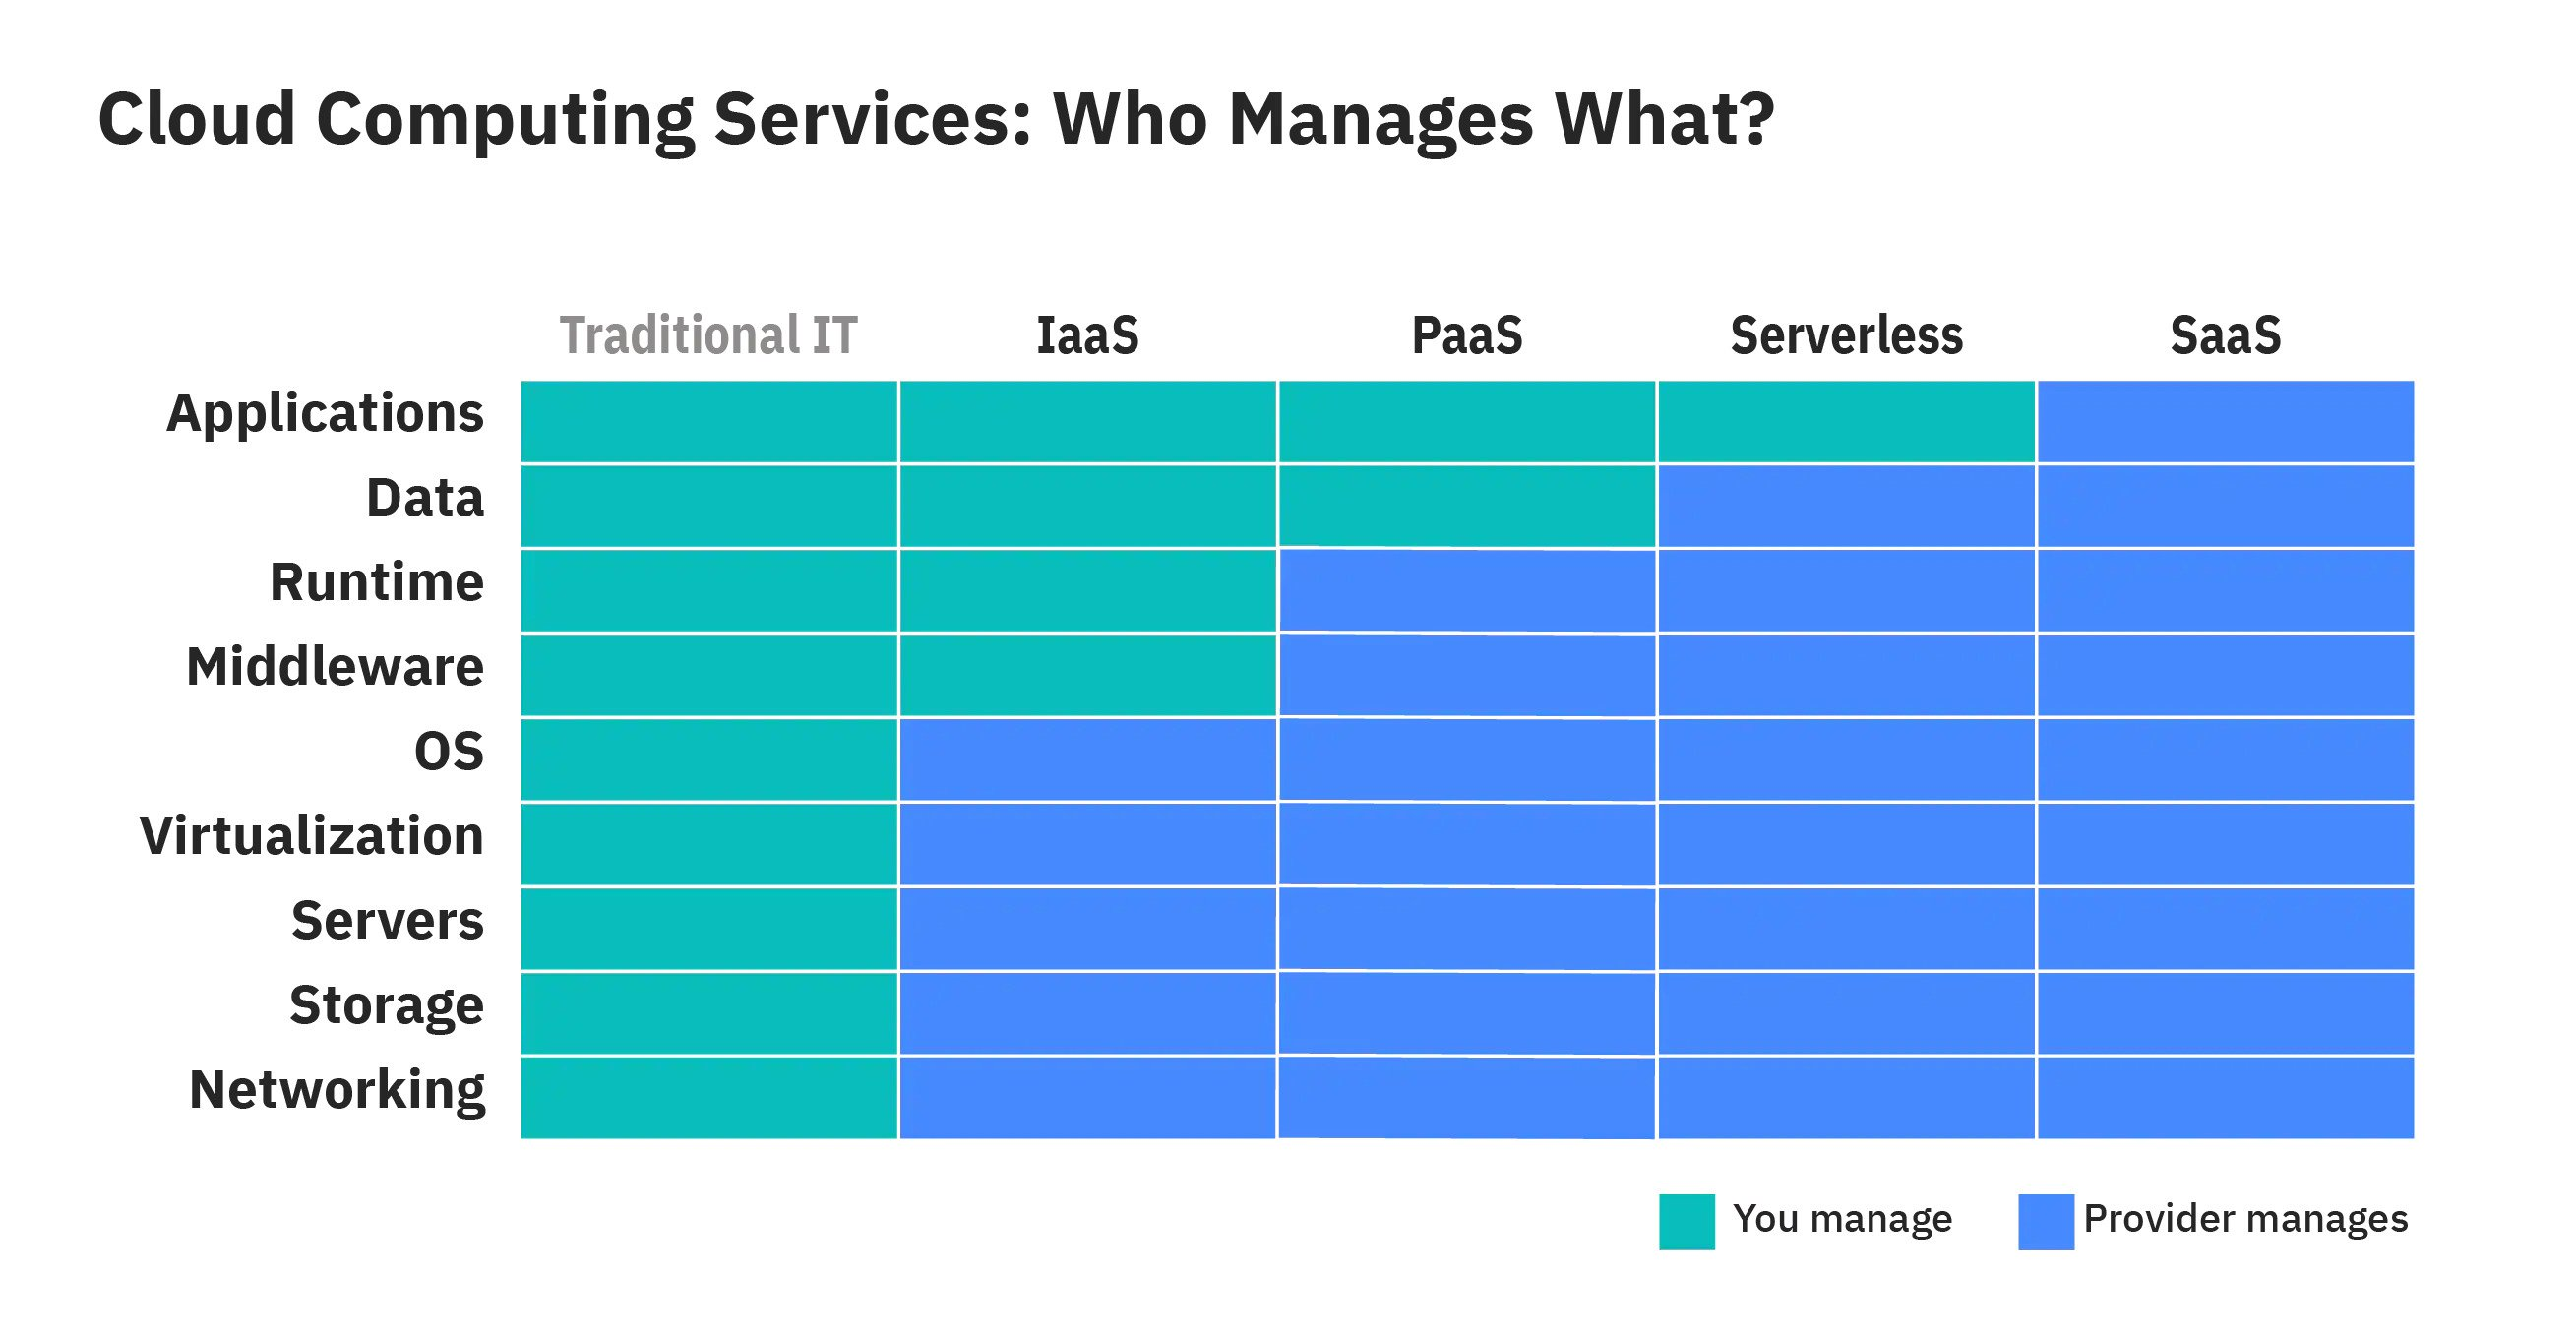
\includegraphics[width=120mm]{ibm.jpg}

\section{Συμπεράσματα - Επισημάνσεις}
Το συμπέρασμα από αυτή τη μελέτη όσον αφορά για τον αντίκτυπο του Νέφους στην κοινωνία:
\begin{itemize}
\item Μεγάλες και μικρομεσαίες επιχειρήσεις μπορούν να μετατρέψουν τις ιδέες τους σε επιχειρηματικά αποτελέσματα, πιο γρήγορα και χωρίς υπερβολικό κόστος.
\item Οι προγραμματιστές μπορούν να αφοσιωθούν στη επιχειρηματική λογική, αντί να ασχολούνται με περίπλοκες διαδικασίες που αφορούν τη διαχείριση του Υλικού.
\item	Οι απλοί χρήστες μπορούν να έχουν πρόσβαση στις διάφορες εφαρμογές από οποιαδήποτε συσκευή και να απολαμβάνουν άπειρες χρήσιμες υπηρεσίες.
\end{itemize}
Γενικότερα μέσα από την εργασία αυτή εξετάσαμε τα νέα δεδομένα στον χώρο των πληροφοριακών συστημάτων, τις νέες ανάγκες για συλλογή και διαχείριση πληροφορίας όπως αυτές προκύπτουν απο τις κοινωνικοοικονομικές αλλαγές που βιώνουμε και το πως τα σύγχρονα πληροφοριακά συστήματα θα πρέπει να τις καλύψουν. Εξετάσαμε τον ρόλο του Υπολογιστικού Νέφους στα παραπάνω, τα πλεονεκτήματα και τα μειονεκτήματά του. Αναζητήσαμε πληροφορίες για τα μοντέλα που το απαρτίζουν, τα πλεονεκτήματα και τα μειονεκτήματά τους, σε ποιές περιπτώσεις μπορούν να φανούν χρήσιμα. Μέσα από τα παραπάνω αποκτήσαμε πολύ καλή κατανόηση των λύσεων αλλά και των προκλήσεων που φέρνει το Υπολογιστικό Νέφος στο τραπέζι, ιδιαίτερα σε σχέση με την συλλογή και διαχείριση πληροφορίας, και θεωρούμε πως το Υπολογιστικό Νέφος θα παίξει καθοριστικό ρόλο στη μελλοντική ανάπτυξη των πληροφοριακών συστημάτων, ιδιαίτερα κάνοντας τα πιο προσβάσιμα σε μικρές και μεσαίες επιχειρήσεις και οργανισμούς.

\section{Βιβλιογραφικές Αναφορές}
\selectlanguage{english}
\begin{itemize}
    \item Al Shehri, Waleed. (2013). Cloud Database Database as a Service. International Journal of Database Management Systems.
    \item Red Hat (2020). IaaS Vs PaaS Vs SaaS
    \item IBM Cloud Learn Hub
    \item Cameron Bassett (2015). Cloud computing and innovation: its viability, benefits, challenges and records management capabilities
    \item Carter, Brian. (2016). Grow your own Backend-as-a-Service (BaaS) platform. 
    \item Cloud Computing Course slides of Sapienza University of Rome
    \item Oleksii, Glib. (2021). Backend as a Service (BaaS): What is it and Key Benefits.
    \item Albugmi, Ahmed & Alassafi, Madini & Walters, Robert & Wills, Gary. (2016). Data Security in Cloud Computing.
    \item Fox, Geoffrey & Isahagian, Vatche & Muthusamy, Vinod & Slominski, Aleksander. (2017). Status of Serverless Computing and Function-as-a-Service(FaaS) in Industry and Research. 
    \item Bodden, Eric. (2015). (In)Security of Backend-as-a-Service
\end{itemize}

\end{document}
